\documentclass[11pt]{article}
\usepackage[T1]{fontenc}
\usepackage[utf8]{inputenc}
\usepackage{lmodern}
\usepackage[margin=1in]{geometry}
\usepackage{microtype}
\usepackage{amsmath,amssymb,amsthm,mathtools}
\usepackage{enumitem,booktabs,array}
\usepackage{needspace}
\usepackage{tikz}
\usetikzlibrary{arrows.meta,positioning,calc,fit,backgrounds,matrix,decorations.pathreplacing}
\usepackage[numbers,sort&compress]{natbib}
\PassOptionsToPackage{hyphens}{url}
\usepackage[colorlinks=true,linkcolor=blue!55!black,citecolor=blue!55!black,urlcolor=blue!55!black]{hyperref}
\usepackage[capitalise,noabbrev]{cleveref}
\hypersetup{pdftitle={Finite tensor savings and exact Fourier circuits},pdfauthor={OpenAI}}
\ifdefined\pdfinfoomitdate\pdfinfoomitdate=1\fi
\ifdefined\pdftrailerid\pdftrailerid{}\fi
\ifdefined\pdfsuppressptexinfo\pdfsuppressptexinfo=15\fi
\setlength{\emergencystretch}{2em}
\numberwithin{equation}{section}
\newtheorem{theorem}{Theorem}[section]
\newtheorem{lemma}[theorem]{Lemma}
\newtheorem{proposition}[theorem]{Proposition}
\newtheorem{corollary}[theorem]{Corollary}
\theoremstyle{definition}
\newtheorem{definition}[theorem]{Definition}
\newtheorem{example}[theorem]{Example}
\theoremstyle{remark}
\newtheorem{remark}[theorem]{Remark}
\newcommand{\C}{\mathbb C}
\newcommand{\R}{\mathbb R}
\newcommand{\N}{\mathbb N}
\newcommand{\Id}{I}
\newcommand{\eps}{\varepsilon}
\DeclareMathOperator{\GL}{GL}
\DeclareMathOperator{\Mat}{Mat}
\DeclareMathOperator{\diag}{diag}
\DeclareMathOperator{\rank}{rank}
\DeclareMathOperator{\tr}{tr}
\DeclareMathOperator{\supp}{supp}
\DeclareMathOperator{\nnz}{nnz}
\DeclareMathOperator{\im}{im}
\DeclareMathOperator{\Span}{span}
\DeclareMathOperator{\poly}{poly}
\title{Finite tensor savings and exact Fourier circuits}
\author{OpenAI}
\date{September 25, 2026}
\begin{document}
\maketitle
\begin{abstract}
We construct exact nonuniform Fourier circuits of size $o(n\log n)$ along an
unbounded sequence of lengths, counting every addition, subtraction, and scalar
multiplication. This refutes the $\Omega(n\log n)$ lower bound in the unrestricted
complex linear-circuit model. The construction uses a finite tensor saving:
a tensor power of some invertible nonmonomial complex matrix can be computed
with fewer matrix calls than the standard tensor-axis algorithm on the same
coordinates, when invertible monomial maps are allowed freely between calls.
\end{abstract}
\tableofcontents
\section{Introduction}\label{intro:sec:introduction}

The discrete Fourier transform is a basic test case for arithmetic
complexity. Its familiar $O(n\log n)$ algorithms make the corresponding
lower-bound question particularly sharp: does every exact computation
require a constant multiple of $n\log n$ operations? The answer depends
on the computational model. We consider complex linear circuits with
arbitrary prechosen coefficients and prove that this lower bound is
false in its unrestricted nonuniform form.

The argument centers on a finite question about tensor products.
For integers $q,b\ge2$, applying a fixed $q\times q$ matrix on each axis
computes its $b$th tensor power with $bq^{b-1}$ matrix calls.
A \emph{monomial matrix} is a permutation matrix times an invertible
diagonal matrix. We prove that, for at least one invertible nonmonomial
matrix, an exact computation improves this
count. A single such finite saving is enough: tensor amplification
turns it into an exponent improvement, and a factorization that preserves
the number of coordinates transfers the improvement to Fourier matrices.
The existence proof develops a second set of tools, based on prices of
matrix calls and their behavior under feedback and changes of boundary
conditions.

\subsection{The model and the result}

For $n\ge2$, put $\zeta_n=\exp(2\pi i/n)$ and let
\begin{equation}\label{intro:eq:fourier}
 F_n=(\zeta_n^{jk})_{0\le j,k<n}.
\end{equation}
A linear circuit has inputs $x_0,\ldots,x_{n-1},0$ and a finite directed
acyclic graph of scalar gates. Each gate computes $u+v$, $u-v$, or
$\lambda u$ from previously available values, with a fixed
$\lambda\in\C$. Each such gate costs one operation, including every
scalar multiplication. Previously computed values can be reused
arbitrarily, and the outputs are designated available values. A fixed
combination $\alpha u+\beta v$ therefore costs at most three gates.

The graph and coefficients may depend on $n$, but not on the input.
Coefficients have no bound on magnitude, algebraic degree, or description
length; their generation is not charged. Depth, storage, cancellation,
and conditioning are unrestricted. All $n$ output coordinates must equal
$F_nx$ exactly for every $x\in\C^n$. Let $L(n)$ be the minimum number of
gates in such a circuit.

\Needspace{8\baselineskip}
\begin{theorem}\label{thm:main}
In this model,
\[
 \liminf_{n\to\infty}\frac{L(n)}{n\log_2 n}=0.
\]
Equivalently, for every $c>0$ and every integer $N_0\ge2$, there is an
integer $n\ge N_0$ and an exact circuit for $F_n$ with fewer than
$c n\log_2 n$ gates.
\end{theorem}

The $\Omega(n\log n)$ Fourier lower-bound question is discussed in
\citet[Abstract]{ailon2013} and \citet[Section~1]{almanRao2023}.
In the model above, \cref{thm:main} refutes the assertion that
$L(n)\ge c n\log_2 n$ for some fixed $c>0$ and all sufficiently large $n$.
The proof gives an unbounded sequence of
lengths, formed as products of distinct primes, with a vanishing
normalized gate count. It is an existence theorem in the stated
nonuniform model. The coefficients are chosen separately for each
resulting circuit; their preparation is outside this model. The theorem
concerns arithmetic operation counts along those lengths and makes no
assertion about coefficient size, numerical stability, or bit complexity.
Neither a uniform construction nor an all-length upper bound is needed
for this quantified conclusion.

\subsection{Historical context}

The fast Fourier transform of Cooley and Tukey organizes a composite-length
transform into smaller transforms and diagonal factors
\citep{cooleyTukey1965}. Coprime factors have a particularly useful
structure: Chinese remainder permutations identify the transform with a
tensor product without intervening diagonal factors. This is the
Good--Thomas factorization; Good's treatment gives the multidimensional
and coprime formulas, and Cooley, Lewis, and Welch describe Thomas's
construction and its relation to Good's work
\citep[Sections~11--12]{good1958}
\citep[pp.~1675--1677]{cooleyLewisWelch1967}.
Convolution supplies another classical route to general lengths.
The 1969 chirp-transform paper of Rabiner, Schafer, and Rader derives
the reduction to diagonal scalings and a convolution, crediting
Bluestein's 1968 work for the quadratic-exponent identity
\citep[Section~II]{rabinerSchaferRader1969}. Bluestein's journal treatment
appeared in 1970 \citep{bluestein1970}.
The transfer proved here uses the coprime tensor structure together with
a local factorization on exactly the original coordinates. Preserving
that width is what permits a finite tensor saving to survive synchronization.

Lower bounds have been proved under substantial restrictions on the
algorithm. Morgenstern's determinant argument establishes a bound of
order $n\log n$ for the unnormalized transform in a bounded-coefficient
model \citep{morgenstern1973}. Ailon proves a lower bound for the
normalized transform in a model with exactly $n$ registers and unitary
$2\times2$ gates \citep[Section~2 and Theorem~2.1]{ailon2013} and, in a
separate model, relates the operation count to the conditioning of
every intermediate transformation
\citep[Definition~2.1 and Theorem~3.1]{ailon2014}.
Those hypotheses are significant here:
the circuits in \cref{thm:main} are allowed arbitrary coefficients and
arbitrary intermediate conditioning.
An unrestricted scalar circuit can pass between normalized and
unnormalized transforms with $O(n)$ additional gates. Such a scaling
need not respect a prescribed coefficient bound, so the normalization
must be retained when comparing the restricted models.

Upper bounds have also improved within the $n\log n$ scale. In particular,
Alman and Rao obtain new leading constants for power-of-two transforms,
measured in real arithmetic operations \citep[Theorem~1.2]{almanRao2023}.
A fixed leading-constant improvement
does not settle the quantified question addressed here. The essential
step in this paper is to turn one strict finite tensor saving into a
smaller exponent in the tensor order, and then preserve that saving
when passing to an unbounded sequence of Fourier transforms.

Tensor amplification and duality also appear in recent work on
Kronecker-power circuits. Alman and Li use asymptotic-spectrum duality
to characterize the asymptotic size of depth-two linear circuits
\citep[Sections~1.3 and~4]{almanLi2025}. Their circuits are represented by rank-one
decompositions, with size measured by the nonzero entries in the two
matrix factors. Our finite-win question concerns sequential invertible
matrix calls on a fixed coordinate set. Its price construction must
therefore preserve the order of each program while combining different
matrix types.

The local Fourier construction uses established ideas from structured
linear algebra and reversible computation. Kuznetsov gives an
$LDL^{\mathsf T}$ factorization of geometric Vandermonde matrices,
including Fourier matrices, whose triangular factors are diagonal
scalings of triangular Toeplitz matrices
\citep[Theorem~1]{kuznetsov2018}. We give a Newton-polynomial derivation
of this identity and implement its factors on the original coordinates.
Low displacement rank supplies the convolution representation used in
that implementation \citep[Lemmas~1--2]{kailathKungMorf1979}.
Computing, reading the output, and reversing a computation is the
uncomputation pattern of Bennett \citep[pp.~526--529]{bennett1973}.
Restoration from arbitrary workspace contents is achieved by the
cleanup construction for transparent programs
\citep[Section~3]{buhrmanEtAl2014}. We prove the particular linear
replay identity, its pair-layer bound, and its fit inside the existing
coordinate set.

The companion manuscript \emph{An explicit power saving for the exact
discrete Fourier transform} gives a quantitative all-length algorithm
in a model that also charges scalar preparation and logarithmic-word
address operations, with a specified root of unity supplied
\citep[Theorem~1.1]{openaiExplicitFourier2026}.
The present paper develops the general finite-win existence argument:
comparison packing, the resulting price laws, and the reflection
contradiction are proved in full independently of that algorithm.

\subsection{The mechanism of the proof}

For an invertible $q\times q$ matrix $A$, the usual computation of
$A^{\otimes b}$ uses $bq^{b-1}$ calls to $A$, acting along tensor fibers.
Call a strict improvement a \emph{finite win}: an exact word on $q^b$
coordinates, using fewer calls, with permutations and invertible
diagonal maps allowed between them. The matrix $A$ must be nonmonomial.
This intermediate convention is confined to matrix words. Every scalar
multiplication is charged when such a word is implemented as a circuit.

The argument has two parts.

\begin{enumerate}[leftmargin=*,label=\textup{(\roman*)}]
\item \emph{A finite win implies \cref{thm:main}.}
For any nonmonomial $A$, one fixed positive-call pattern, with adjustable
monomial factors, realizes every invertible matrix of the same width.
A finite win then gives circuits for $A^{\otimes k}$ with
$O(q^k(k+1)^\alpha)$ gates for some fixed $\alpha<1$.
Each Fourier matrix $F_r$ is factored, on its original $r$ coordinates,
into $O(1+\log^4 r)$ layers, each monomial or a disjoint union of
invertible two-coordinate maps with any remaining coordinates fixed.
The temporary convolution computations
borrow arbitrary existing values and restore them by cancellation.
Positive generation places the pair maps in fixed-width tuples and
replaces them by a common call pattern in $A$. Synchronizing this pattern
across distinct prime factors makes each call slot a direct sum of
tensor powers of $A$. The sector widths sum to the Fourier length, so
the amplified bound controls the entire slot. The Chinese Remainder
Theorem then gives the desired sequence.

\item \emph{A finite win must exist.}
Suppose that none exists. Compare tensor-axis computations with words
using a finite collection of matrix types. If several comparisons
together save calls to every type, we can place their programs on
disjoint tensor sectors and schedule them as calls to one larger
block-diagonal matrix. This would give a finite win. Separation and
compactness turn the impossibility of such simultaneous savings into
one price function $p$, positive on nonmonomial matrices, with exact tensor
and direct-sum laws.

We next ask how prices change when coordinates are eliminated. Split
the coordinates of an invertible matrix into data and state, and apply
it repeatedly to fresh data while retaining the state. Repeat this
construction on many tensor axes. The cost of correcting the initial
state becomes negligible compared with the number of cell calls. This
proves that an invertible corner costs no more than its
containing matrix. Comparing multiplication modulo different scalar
polynomials also permits closing the state connection and specializing
rational matrix families. All these conclusions concern exact matrices;
they do not assume continuity of the price.

Finally, normalize a nontrivial elementary shear to have price one.
A legal exchange of one input basis member with one output basis member
preserves price, provided both exchanged lists remain bases. Applying
these exchanges to signed bit-coordinate matrices gives a family of
involutions, with integer parameter $d$, width $w=w(d)$, and price $dw$.
The constructed $+1$ eigenspace is the graph of an invertible matrix.
From the orthogonal reflection $R$ in that graph, we can recover the
involution's price at an additional cost of only $O(w)$.
The same subspace is the kernel of a real symmetric matrix with at most
$(d/2+1)w$ supported off-diagonal pairs. A product of diagonal and
two-coordinate perturbations has this sparse matrix as its derivative
at zero. At generic parameter values, each dense pair costs at most
$3/2$. Feedback adds only $O(w)$, and two algebraic specializations
carry the bound to $R$. Thus the two descriptions give
\[
 dw-O(w)\leq p(R)\leq \frac{3d}{4}w+O(w),
\]
with absolute implied constants. They are incompatible for sufficiently
large $d$.
\end{enumerate}

These parts meet at one precise interface: the finite word of
\cref{def:finite-win}. The transfer in \cref{prop:win-to-fourier} works
for any word satisfying that definition, while
\cref{thm:finite-win} establishes that at least one exists. In particular,
the proof does not require a finite win for every nonmonomial matrix.

\subsection{Conventions and order of the argument}

All matrices and scalar coefficients are over $\C$, except where real
symmetry and real orthogonality are explicitly used. Tensor products are
ordinary Kronecker products. For an invertible square
matrix $A$, its width is denoted by $|A|$. A matrix call acts on an ordered
tuple of distinct coordinates and fixes every other coordinate.
Zero-dimensional blocks may be omitted. A superscript $\mathsf T$
denotes ordinary transpose, not conjugate transpose.

The price function is introduced only under the assumption that there
is no finite win. It is an auxiliary real-valued function, not an
asserted lower bound for circuit size. Every limiting argument proves
an inequality for exact finite matrices. In particular, specialization
never replaces an exact circuit by a limit of approximate computations.

Constants in an $O$ bound may depend on fixed local matrices and their
dimensions. When a tensor order $k$ and a run length $t$ vary, each
polynomial bound in $k$ has a fixed exponent and is independent of $t$
unless stated otherwise. Scalar coefficients may depend on these
parameters, as the model permits. We specify the order of choices at
the packing, feedback, and specialization steps.

\Cref{gen:sec:generation,fft:transfer} prove the transfer from one finite
win, through positive generation, amplification, and exact-width Fourier
layers. \Cref{price:section} constructs the price function from the
opposite assumption. \Cref{corner:sec:corners,feedback:sec} establish
corner contraction, feedback, and algebraic specialization.
\Cref{pivot:sec:pivots} gives scalar-pivot invariance and the dense-pair
bound. Finally, \cref{reflect:section} uses those laws to force the
reflection contradiction and prove \cref{thm:finite-win}, which closes
the proof of \cref{thm:main}.

\section{Positive words and tensor amplification}
\label{gen:sec:generation}

For an invertible square matrix $A$, write $|A|$ for its width.
A \emph{monomial matrix} is a permutation matrix times an invertible
diagonal matrix.  A \emph{call to $A$ on $w$ coordinates}, where $w\geq
|A|$, applies $A$ to an ordered tuple of $|A|$ distinct coordinates and
fixes the others.  A \emph{matrix word} is a finite composition of such
calls and full-width monomial matrices.  In a word using one specified
matrix $A$, its \emph{call count} counts only occurrences of $A$;
monomials have zero call count.  This convention concerns words alone.
In the scalar circuit model, a monomial on $w$ coordinates costs at most
$w$ scalar multiplications, with its permutation realized by designating
the appropriate available values.

\begin{definition}[Finite win]\label{def:finite-win}
A finite win consists of an invertible nonmonomial matrix
$A\in\GL_q(\C)$, an integer $b\geq2$, and a word on exactly $q^b$
coordinates implementing $A^{\otimes b}$ with $g$ calls to $A$, where
\begin{equation}\label{gen:eq:strict-win}
g<bq^{b-1}.
\end{equation}
\end{definition}

The comparison in \cref{gen:eq:strict-win} is with the usual tensor-axis
algorithm: for each of the $b$ axes, it makes $q^{b-1}$ calls to $A$.
Nonmonomiality implies $q\geq2$.  It also implies that $A^{\otimes b}$
is nonmonomial: an invertible nonmonomial matrix has a row with at least
two nonzero entries, and tensoring that row with any nonzero rows
preserves this property.  Thus a winning word necessarily has $g\geq1$.

\subsection{One fixed positive pattern generates every target}

The following statement supplies both the local substitutions in the
Fourier transfer and positive-call identity words used later in packing.
The positions of all calls are fixed before the target matrix is chosen.

\begin{samepage}
\begin{lemma}[Positive generation]\label{lem:generation}
Let $A\in\GL_q(\C)$ be nonmonomial.  There is an integer $h>0$ such that
every $H\in\GL_q(\C)$ admits a factorization
\begin{equation}\label{gen:eq:common-pattern}
H=M_0 A M_1 A\cdots A M_h,
\end{equation}
with exactly $h$ occurrences of $A$ and monomial matrices $M_i$.
In particular, identity admits such a factorization with a positive
number of calls.  More generally, for every fixed $w\geq q$, there is
a fixed positive pattern on $w$ coordinates realizing every element
of $\GL_w(\C)$ by embedded calls to $A$ and monomials.
\end{lemma}
\end{samepage}

\begin{proof}
We build a fixed word whose adjustable diagonal factors give a full-rank
differential, then show that its actual values contain a nonempty Zariski
open subset of $\GL_q(\C)$.  Every invertible target is a product of two
values from this subset, so doubling the word gives the common pattern.

Let $E_{ij}$ denote the matrix units.  Let
$\mathfrak d\subset\Mat_q(\C)$ be the diagonal subspace and let
$\mathcal S$ be the semigroup of words in $A$ and monomials, including
identity.  Inverses are not among the specified calls.  First we prove
\begin{equation}\label{gen:eq:tangent-span}
\Span_{s\in\mathcal S}s\mathfrak d s^{-1}=\Mat_q(\C).
\end{equation}
If $A\mathfrak d A^{-1}\subset\mathfrak d$, each rank-one idempotent
$A E_{ii}A^{-1}$ would be a diagonal rank-one idempotent, hence some
$E_{\pi(i)\pi(i)}$.  Orthogonality of these idempotents forces $\pi$
to be a permutation.  The identity
$A E_{ii}=E_{\pi(i)\pi(i)}A$ then says that column $i$ of $A$ is
supported in row $\pi(i)$; invertibility would make $A$ monomial.
Consequently some $X\in A\mathfrak d A^{-1}$ has $X_{ij}\ne0$ for
$i\ne j$.

Write $\mathcal V$ for the span on the left of
\cref{gen:eq:tangent-span}.  For every invertible diagonal
$D=\diag(d_1,\ldots,d_q)$, the matrix $DXD^{-1}$ belongs to $\mathcal V$.
If a linear functional $\ell$ vanishes on $\mathcal V$, then
\[
0=\ell(DXD^{-1})
 =\sum_a X_{aa}\ell(E_{aa})
  +\sum_{a\ne c}X_{ac}\ell(E_{ac})d_a/d_c
\qquad(d_1,\ldots,d_q\in\C^*).
\]
The Laurent monomials $1$ and $d_a/d_c$ for $a\ne c$ are distinct and
linearly independent.  Thus $X_{ij}\ell(E_{ij})=0$, and so
$\ell(E_{ij})=0$.  Finite-dimensional linear duality gives
$E_{ij}\in\mathcal V$.  Conjugation by any permutation preserves
$\mathcal V$, because left multiplication of a word by that permutation
is again a word.  Hence $\mathcal V$ contains every off-diagonal matrix
unit.  It also contains $\mathfrak d$, using $s=I_q$.  This proves
\cref{gen:eq:tangent-span}.

We next arrange the spanning directions along one word.  Start with
the prefix $h_0=I_q$ and its diagonal directions.  If the directions
collected so far span a proper subspace and the current prefix is $h$,
then
\[
\Span_{s\in\mathcal S}(hs)\mathfrak d(hs)^{-1}
 =h\Mat_q(\C)h^{-1}=\Mat_q(\C).
\]
Choose a word $s$ whose directions enlarge the collected span, and
append it to the right of $h$ in written product order.  Each choice
increases the dimension, so finitely many choices suffice.  Denote the
successive appended words by $s_1,\ldots,s_r$ and their prefixes by
$h_i=s_1\cdots s_i$.  The spaces $h_i\mathfrak d h_i^{-1}$, including
$i=0$, now span $\Mat_q(\C)$.

Insert variable diagonal factors in the product
\[
\Phi(D_0,\ldots,D_r)=D_0s_1D_1s_2\cdots s_rD_r.
\]
At $D_0=\cdots=D_r=I_q$, its value is $h_r$.  Varying $D_i$ in the
diagonal direction $E_{aa}$ gives the right-translated derivative
\[
(\delta\Phi)h_r^{-1}=h_iE_{aa}h_i^{-1}.
\]
Thus the derivative has rank $a=q^2$.  Choose $a$ diagonal entries
whose derivative columns are independent, and fix all other entries
to $1$.  Listing matrix entries produces a polynomial map
\[
f:\C^a\longrightarrow\C^a
\]
whose Jacobian determinant is nonzero at $(1,\ldots,1)$.  Parameters in
$(\C^*)^a$ give admissible words.  We show next that their image contains
an actual nonempty Zariski open subset of $\GL_q(\C)$.

Write $x_1,\ldots,x_a$ for the selected parameters and
$f_1,\ldots,f_a$ for the output entries.  The $f_i$ are algebraically
independent.  Indeed, a nonzero polynomial relation $P(f)=0$ of least
total degree would, upon differentiation and inversion of the Jacobian
over $\C(x_1,\ldots,x_a)$, imply
$(\partial P/\partial y_i)(f)=0$ for every $i$.  In characteristic zero
at least one of these is a nonzero polynomial of smaller degree,
a contradiction.  Both fields in the inclusion
\[
\C(f_1,\ldots,f_a)\subset\C(x_1,\ldots,x_a)
\]
therefore have transcendence degree $a$.  The latter is an algebraic
extension generated by the finitely many $x_i$, so it is finite.
Each of the finitely many
elements $x_i,x_i^{-1}$ satisfies a monic equation over the smaller
field.  Choose a nonzero polynomial $g(y_1,\ldots,y_a)$ divisible by
the denominators of all coefficients of these equations.  With
\begin{align*}
R&=\C[f_1,\ldots,f_a,1/g(f)],\\
B&=R[x_1,\ldots,x_a,x_1^{-1},\ldots,x_a^{-1}]
   \subset\C(x_1,\ldots,x_a),
\end{align*}
all the displayed generators of $B$ are integral over $R$.
Reducing their powers by their monic equations shows directly that
$B$ is a finite $R$-module.  Both are domains and $R\hookrightarrow B$
is injective.  This is the finite-type integral-extension criterion
\citep[Tag~02JJ, Lemma~10.36.5]{stacksProject}.

Fix any target $y\in\C^a$ with $g(y)\ne0$, and let
$\mathfrak m=(f_1-y_1,\ldots,f_a-y_a)\subset R$.  Algebraic independence
identifies $R/\mathfrak m$ with $\C$.  Localizing the inclusion above
gives $R_{\mathfrak m}\hookrightarrow B_{\mathfrak m}$ inside the field
$\C(x_1,\ldots,x_a)$, so $B_{\mathfrak m}$ is a nonzero finite module
over the local ring $R_{\mathfrak m}$.  Its residue algebra
\begin{equation}\label{gen:eq:nonzero-fiber}
B_{\mathfrak m}/\mathfrak mB_{\mathfrak m}
\end{equation}
is nonzero.  This is the lying-over step for the integral inclusion
\citep[Tag~00GQ, Lemma~10.36.17]{stacksProject}.
For completeness, if it were zero, a finite list of module
generators $b_1,\ldots,b_e$ would satisfy
$b_i=\sum_j c_{ij}b_j$ with all $c_{ij}$ in the maximal ideal of
$R_{\mathfrak m}$.  The determinant of $I-(c_{ij})$ is a unit in this
local ring.  Multiplication by its adjugate forces every $b_i$ to be
zero, contradicting $B_{\mathfrak m}\ne0$.

The algebra in \cref{gen:eq:nonzero-fiber} is finite dimensional over
$\C$.  A quotient by a maximal ideal is a finite field extension of
$\C$, and hence is $\C$ itself.  The resulting homomorphism
$B\to\C$ sends $x_i$ to some $\xi_i\ne0$, since $x_i^{-1}$ is also in
$B$.  The polynomial identities defining the $f_i$ descend to
$f_i(\xi)=y_i$.  These are actual admissible parameters of the fixed
word.  In particular its image contains
\[
\Omega=\{Y\in\Mat_q(\C):g(Y)\det Y\ne0\},
\]
a nonempty open set, because $g(Y)\det Y$ is a nonzero polynomial.

Finally fix $H\in\GL_q(\C)$.  There is a $V$ for which both
$V\in\Omega$ and $V^{-1}H\in\Omega$.  To see this without any limiting
argument, clear powers of $\det V$ from $g(V^{-1}H)$.  Its numerator is
a nonzero polynomial: the substitution $V\mapsto V^{-1}H$ is a
bijection of $\GL_q(\C)$, with inverse $W\mapsto HW^{-1}$, so this
rational function is not identically zero.  Avoid simultaneously the
zeros of that numerator, $g(V)$, and $\det V$.  A finite product of
nonzero polynomials over $\C$ is nonzero and has a point where it does
not vanish.  This supplies the required $V$.  Setting $W=V^{-1}H$
gives $H=VW$, with both factors realized by the same fixed word
pattern.  Two copies of that pattern therefore realize every $H$.

The initial pattern contains at least one occurrence of $A$: otherwise
its values have one fixed monomial support, a space of dimension $q$,
contradicting the derivative rank $q^2>q$.  Expanding the fixed words
$s_i$ and merging adjacent monomials in the doubled pattern gives
\cref{gen:eq:common-pattern} with a fixed $h>0$.  All inverses used in
the argument occurred in matrix identities or parameter selection;
every factor of the constructed words is a forward call to $A$ or a
monomial.  For $w>q$, applying the same result to the nonmonomial matrix
$A\oplus I_{w-q}$ proves the wider-width assertion, because each call
to this matrix is one embedded call to $A$.
\end{proof}

\subsection{Amplifying a finite saving}

The next lemma concerns scalar gates, including the cost of every
monomial scaling.  All its constants are allowed to depend on the
single fixed finite win.

\begin{lemma}[Tensor amplification]\label{lem:amplification}
If $(A,b,g)$ and a specified winning word form a finite win, then there
are constants $C<\infty$ and $0<\alpha<1$ such that $A^{\otimes k}$ has
an exact scalar linear circuit with at most
$Cq^k(k+1)^\alpha$ gates for every integer $k\geq0$.
\end{lemma}

\begin{proof}
Let $L_A(k)$ be the minimum scalar gate count for $A^{\otimes k}$,
and put $f(k)=L_A(k)/q^k$.  Here $A^{\otimes0}=I_1$ and $f(0)=0$.
These minima exist: entrywise multiplication and addition give finite
circuits, and a nonempty set of nonnegative integer gate counts has
a minimum.  Set
\[
Q=q^b,\qquad p=q/Q,\qquad j=\lfloor k/b\rfloor.
\]
Tensor the winning word with itself over $j$ groups, multiplying the
corresponding slots together.  The product of these slots is
$(A^{\otimes b})^{\otimes j}=A^{\otimes bj}$.

A monomial slot remains monomial after taking this tensor power, and
therefore costs at most $Q^j$ scalar gates.  Each call slot is
permutation-conjugate to $A\oplus I_{Q-q}$.  Its $j$-fold tensor power,
after reordering coordinates, has the following exact direct-sum
decomposition:
\begin{equation}\label{gen:eq:sector-decomposition}
(A\oplus I_{Q-q})^{\otimes j}
\ \cong\ 
\bigoplus_{r=0}^{j}
\left(A^{\otimes r}\right)^{\oplus
             \binom jr(Q-q)^{j-r}}.
\end{equation}
For a chosen subset of $r$ active factors, the inactive factors supply
$(Q-q)^{j-r}$ independent scalar coordinate choices, explaining the
multiplicity.  The total width is
$\sum_r\binom jr q^r(Q-q)^{j-r}=Q^j$.  Computing the blocks separately
with minimum circuits gives normalized cost at most
\begin{align}
\frac{1}{Q^j}\sum_{r=0}^j
  \binom jr(Q-q)^{j-r}L_A(r)
 &=\sum_{r=0}^j\binom jr p^r(1-p)^{j-r}f(r)\notag\\
 &=\mathbb E f(K),\qquad K\sim\operatorname{Bin}(j,p).
 \label{gen:eq:weighted-cost}
\end{align}
In particular, this distribution weights sectors by their coordinate
dimensions; the sectors have different widths.

Replicate the resulting circuit over the coordinates of the remaining
$k-bj<b$ tensor axes.  The normalized cost is unchanged by this
replication.  If a fixed circuit for $A$ has $\ell_A$ gates, applying
$A$ along each remaining axis costs $\ell_Aq^{k-1}$ gates per axis.
Since the number of monomial slots in the winning word is fixed,
there is a constant $C_0$ independent of $k$ such that
\begin{equation}\label{gen:eq:recurrence}
f(k)\leq C_0+g\,\mathbb E f(K),
\qquad K\sim\operatorname{Bin}(\lfloor k/b\rfloor,q/Q).
\end{equation}
For $j=0$ the grouped part is identity and the same inequality follows
from the bound on the fewer than $b$ remaining axes.  Every permutation
used in deriving \cref{gen:eq:sector-decomposition} is only a
reindexing; every diagonal scaling has already been charged.

Put $\rho=q/(Qb)$.  The strict saving gives $g\rho<1$, and hence we can
choose $0<\alpha<1$ sufficiently close to $1$ that
$g\rho^\alpha<1$.  Choose also a number $\gamma$ with
$g\rho^\alpha<\gamma<1$.  Since
\[
g\left(\frac{\rho k+1}{k+1}\right)^\alpha
 \longrightarrow g\rho^\alpha,
\]
there is $k_0\geq1$ such that this expression is at most $\gamma$ for all
$k\geq k_0$.  Choose $C$ at least $C_0/(1-\gamma)$ and large enough
that $f(k)\leq C(k+1)^\alpha$ for $k<k_0$.
For $k\geq k_0$, every value of $K$ satisfies
$K\leq\lfloor k/b\rfloor<k$.  Strong induction, concavity of
$x\mapsto x^\alpha$, and $\mathbb E K=p\lfloor k/b\rfloor\leq\rho k$
therefore give
\[
f(k)\leq C_0+gC\,\mathbb E(K+1)^\alpha
 \leq C_0+gC(\rho k+1)^\alpha
 \leq C_0+C\gamma(k+1)^\alpha
 \leq C(k+1)^\alpha.
\]
All circuits used in this induction compute exact matrices; the
expectation is merely the finite weighted sum in
\cref{gen:eq:weighted-cost}.  Multiplying by $q^k$ proves the scalar
gate bound
\[
L_A(k)=O\bigl(q^k(k+1)^\alpha\bigr),\qquad 0<\alpha<1.
\]
\end{proof}

\section{From a finite win to exact Fourier circuits}
\label{fft:transfer}

The amplification in \cref{lem:amplification} concerns tensor powers of
one fixed matrix.  To use it for Fourier transforms of different widths,
we first construct shallow matrix words without enlarging those widths.
A \emph{pair layer} is a direct sum, after a coordinate permutation, of
invertible two-coordinate matrices and one-coordinate identities.  A
\emph{monomial layer} is an invertible monomial matrix on the whole
coordinate set.  During a recursive construction we also permit a
\emph{mixed round}: on disjoint regions it performs monomial layers or
pair layers.  Such a round splits into at most two layers of the stated
types, since the operations on different regions commute.

\subsection{Convolutions and borrowed coordinates}

We will use the following elementary circuit fact.  A convolution with a
fixed vector, including truncations and reversals of its inputs or
outputs, has a linear DAG with
\[
 O\bigl(v\log(2+v)\bigr)\quad\text{gates},\qquad
 O\bigl(\log(2+v)\bigr)\quad\text{depth},
\]
where $v$ is the sum of the input and kernel lengths.  Moreover its
variable inputs and gates have bounded fan-out, including uses at the
outputs, with an absolute bound.  Here and below depth counts scalar
arithmetic gates.

For nonempty vectors of lengths $a,e\ge1$, pad both by zeros to the
least power of two $L\ge a+e-1$; then $L<2(a+e-1)$.
Empty operands give the zero map and may be omitted.  At $L=1$ the
Fourier maps are identities.  At
the $L$th roots of unity, ordinary convolution becomes pointwise
multiplication; the transform of the fixed vector is part of the
prechosen constants.  The binary Fourier recursion transforms even and
odd positions separately and combines each pair of transformed entries
$a,b$ as $a+\omega b,a-\omega b$.  It uses at most three scalar gates
per pair, $O(L\log(2L))$ gates in total, and $O(\log(2L))$ depth.
Every recursion input feeds one leaf; each transformed entry is used in
only its own pair of outputs at the next level.  The inverse uses
inverse roots and a final scaling by $L^{-1}$, with the same bounds.
Padding zeros require no variable input.  The intervening diagonal
multiplications and the output selections preserve bounded fan-out.
This also proves the same estimates for a fixed number of such
convolutions, compositions, and sums.  All scalar multiplications in
these estimates are charged.

The padded DAG in this argument need not itself be in place.  The next
lemma explains how its workspace can be supplied by existing
coordinates carrying arbitrary values.
The forward, output, and reverse sweeps follow the uncomputation pattern
of Bennett \citep{bennett1973}. The arbitrary initial values also connect
this construction with transparent computation
\citep[Section~3]{buhrmanEtAl2014}. The second replay below removes their
contribution and supplies the precise shear and layer counts used here.

\begin{samepage}
\begin{lemma}[Dirty-coordinate replay]\label{fft:dirty-layers}
Let $M:\C^e\to\C^a$ have a linear DAG with $\ell$ gates and depth $H$.
Suppose every variable input and gate has fan-out at most $\delta$,
counting designated output uses.  On disjoint source coordinates $x$,
target coordinates $y$, and $\ell$ further coordinates $z$, there is a
word of coordinate shears realizing
\[
 (x,y,z)\longmapsto(x,y+Mx,z).
\]
It uses at most $8\ell+2a$ shears and
$O\bigl((\delta+1)(H+1)\bigr)$ pair layers.  The initial values of $z$
are arbitrary, and may depend on $x,y$ or other data.
\end{lemma}
\end{samepage}

\begin{proof}
Assign one distinct coordinate $z_v$ to each gate $v$, ordered
topologically.  To simulate the gate, add its prescribed linear
combination of predecessors into $z_v$.  A scalar gate requires one
shear, and an addition or subtraction requires at most two.  An edge
from the literal input zero is omitted.  Predecessors are either
original source coordinates or earlier gate coordinates; in particular
none is the coordinate being updated.  The forward sweep therefore
has the form
\begin{equation}\label{fft:dirty-forward}
 z\longmapsto Uz+Tx,
\end{equation}
where $U$ is unit lower triangular in the chosen order.  Write the
designated output reads as $Fz_{\rm current}+Dx$; this includes outputs
that are original inputs, and a zero output contributes no read.  Each
nonzero output is one designated read.  Starting with zero gate
coordinates computes the original DAG, so
\begin{equation}\label{fft:dirty-output}
 FT+D=M.
\end{equation}
Run the forward sweep, add its outputs into $y$, and undo every shear
of that sweep in reverse order.  The net effect on $y$ is addition of
\[
 F(Uz+Tx)+Dx=Mx+FUz,
\]
and every scratch coordinate returns to its initial value.  Next run
the same forward sweep with \emph{all} edges from original source
coordinates omitted.  Omit the direct-source output term $Dx$ as well.
This sweep sends $z$ to $Uz$.  Subtract its outputs $FUz$ from $y$ and
undo the sweep.  This leaves exactly $y+Mx$ and restores $z$ once more.
The target coordinates are never read by either sweep.  These identities
hold for independent formal variables $x,y,z$, hence remain valid after
substituting correlated values for the initial scratch.

To obtain the layer bound, assign gates their longest-path depth
levels.  Within a level, all destinations are new gate coordinates and
all predecessors belong to earlier levels or to the sources.  The
undirected multigraph of shear edges has maximum degree at most
$\Delta=\max\{2,\delta\}$: a destination has at most two incoming
edges and a predecessor has at most $\delta$ uses.  Repeated edges can
be combined, or retained with their bounded multiplicity.  Greedy edge
coloring uses at most $2\Delta-1$ colors, because an edge meets at most
$2\Delta-2$ other edges.  Each color is a disjoint-pair layer.  These
shears can be reordered by colors because no destination in this
level is a predecessor in the same level.  Output additions have the
same bounded-degree property on source or gate coordinates and target
coordinates.  Reversing the colored levels gives the exact inverse
sweep.  Thus four sweeps and two output rounds need at most
$4(2\Delta-1)H+2(2\Delta-1)$ layers.  Each sweep uses at most
$2\ell$ shears and each output round at most $a$, proving the count.
\end{proof}

\subsection{An exact-width factorization}

The structured-matrix step uses the displacement-rank method of Kailath,
Kung, and Morf \citep[Lemmas~1--2]{kailathKungMorf1979}: a matrix whose
difference from a shifted copy has low rank can be reconstructed from
convolution factors. We give the rectangular reconstruction in the proof,
then place its workspace inside the original coordinate set.

\begin{lemma}[Triangular Toeplitz layers]\label{fft:toeplitz-layers}
Every invertible lower triangular Toeplitz matrix of width $r$ has a
factorization on exactly $r$ coordinates into
$O(1+\log^4 r)$ monomial and pair layers.  The implied constant is
absolute and independent of its entries.
\end{lemma}

\begin{proof}
Write $T_r=(h_{i-j})_{0\le j\le i<r}$, with zero entries above the
diagonal and $h_0\ne0$.  Let $g_0,g_1,\ldots$ be the coefficients of
the inverse formal series to $\sum_{j\ge0}h_jz^j$, extending the
specified $h_j$ arbitrarily beyond those needed.  Split at
$s=\lfloor r/2\rfloor$, and put
\[
 T_r=\begin{pmatrix}T_s&0\\ B&T_{r-s}\end{pmatrix}.
\]
First apply its two diagonal blocks recursively and in parallel.  To
finish, add from the first block into the second by $C=BT_s^{-1}$.
With global row and column indices its entries are
\begin{equation}\label{fft:cross-block}
 C_{ij}=\sum_{\nu=j}^{s-1}h_{i-\nu}g_{\nu-j},
 \qquad s\le i<r,\quad 0\le j<s.
\end{equation}

Partition the source and target ranges into consecutive chunks, of a
size to be specified below, and consider a chunk matrix $M$ of size
$a\times e$.  Let $S_a,S_e$ be lower-shift matrices, with ones in
positions $(u,u-1)$.  For entries away from the first row and first
column of the chunk, \cref{fft:cross-block} gives
\[
 M_{uv}-(S_aMS_e^{\mathsf T})_{uv}
 =C_{ij}-C_{i-1,j-1}=-h_{i-s}g_{s-j}.
\]
The right side is an outer product on those entries.  Extending this
outer product to the whole chunk leaves only its first row and first
column to correct; these have rank at most one each.  Consequently
\begin{equation}\label{fft:displacement}
 E=M-S_aMS_e^{\mathsf T}
   =\sum_{\nu=1}^{\rho}v^{(\nu)}(w^{(\nu)})^{\mathsf T},
 \qquad \rho\le3.
\end{equation}
Nilpotence of the shifts gives the terminating telescoping identity
\[
 M=\sum_{l\ge0}S_a^lE(S_e^{\mathsf T})^l.
\]
For one outer product $vw^{\mathsf T}$ its summand matrix has entries
$\sum_{l\ge0}v_{u-l}w_{j-l}$, with both vectors zero-extended.
It applies to $x\in\C^e$ by the two maps
\begin{equation}\label{fft:two-convolutions}
 b_l=\sum_{j=l}^{e-1}w_{j-l}x_j\quad(0\le l<e),
 \qquad
 c_u=\sum_{l=0}^{e-1}v_{u-l}b_l\quad(0\le u<a).
\end{equation}
The first is a convolution after reversing the input and selecting
coefficients; the second is a truncated convolution.  Sum the at most
three resulting vectors.  The preceding binary-FFT construction
therefore supplies a DAG for $Mx$ satisfying, for absolute constants
$C_0,C_1,\delta_0$,
\begin{equation}\label{fft:chunk-dag}
 \ell\le C_0(a+e)\log_2(2+a+e),\qquad
 H\le C_1\log_2(2+a+e),\qquad
 \delta\le\delta_0.
\end{equation}
These bounds include the sums of the at most three terms and all
output uses.  In particular, copying the input to these three fixed
networks multiplies its fan-out by only a constant.  The constants do
not depend on the Toeplitz entries or the chosen outer products.

Choose once and for all $D\ge16C_0+16$ and, for sufficiently large
$r$, take chunk size
\[
 h=\left\lfloor\frac{r}{D\log_2r}\right\rfloor.
\]
Choose a fixed threshold $r_0$ so that, for all $r\ge r_0$,
$h\ge r/(2D\log_2r)\ge1$.  The final chunk in either range may be
shorter.  For every chunk pair,
\[
 a+e\le\frac{2r}{D\log_2r}\le\frac r8,
 \qquad
 \log_2(2+a+e)\le2\log_2r,
 \qquad
 \ell\le\frac{4C_0r}{D}<\frac r4.
\]
At least $7r/8$ coordinates of this very recursion block lie outside
the source and target chunks.  They suffice for the $\ell$ scratch
coordinates in \cref{fft:dirty-layers}.  No extra coordinate is
introduced for the padded FFT: its zero inputs require no register,
and every gate requiring a register is already counted in $\ell$.
The lemma implements addition of this chunk's contribution in
$O(\log r)$ pair layers and restores every other coordinate.

Process the chunk pairs serially.  Source chunks remain unchanged,
target additions accumulate, and coordinates in other chunks can be
borrowed again with their current values, even if already updated.
There are at most $r/h+2=O(\log r)$ chunks in total and hence
$O(\log^2r)$ pairs.  The cross-block update needs
$O(\log^3r)$ layers.  For $r<r_0$, elimination expresses $T_r$ using
scalings and coordinate shears on the same coordinates, at a bounded
cost depending only on the fixed $r_0$.

Let $d(r)$ denote the worst mixed-round depth of this construction.
The child recursions use only their own disjoint blocks, so their
depths take a maximum, and
\[
 d(r)\le\max\{d(\lfloor r/2\rfloor),
                  d(\lceil r/2\rceil)\}
             +O(1+\log^3r).
\]
Summing along the $O(\log r)$ balanced recursion levels gives
$d(r)=O(1+\log^4r)$.  Splitting mixed rounds into at most two layers
finishes the proof, still on exactly $r$ coordinates.
\end{proof}

The Fourier-to-Toeplitz identity used next is the geometric-Vandermonde
$LDL^{\mathsf T}$ factorization of \citet[Theorem~1]{kuznetsov2018},
specialized to a primitive root of unity. For the general Vandermonde
factorization through Newton interpolation, see also
\citet[Theorem~2.1]{orucPhillips2000}. We derive the identity here to fix
our conventions, then apply the preceding layer construction to its
triangular factors.

\begin{lemma}[Exact-width Fourier layers]\label{lem:fourier-layers}
For every integer $r\ge1$, the unnormalized Fourier matrix $F_r$ has
a factorization on exactly $r$ coordinates into
$O(1+\log^4r)$ monomial and pair layers, with an absolute implied
constant.
\end{lemma}

\begin{proof}
The case $r=1$ is identity.  For $r\ge2$ put $u=\zeta_r$, and let
$P$ have as its $k$th column the coefficients of the monic Newton
polynomial $\prod_{j=0}^{k-1}(X-u^j)$, for $0\le k<r$.
Thus $P$ is unit upper triangular.  Evaluating these polynomials gives
$N=F_rP$, a lower triangular matrix, with
\begin{equation}\label{fft:newton}
 N_{ik}=\prod_{j=0}^{k-1}(u^i-u^j)
   =(-1)^k u^{k(k-1)/2}\frac{H_i}{H_{i-k}}\quad(i\ge k),
 \qquad
 H_j=\prod_{e=1}^j(1-u^e),\quad H_0=1.
\end{equation}
Only $H_0,\ldots,H_{r-1}$ occur, all nonzero since $u$ is a primitive
$r$th root.  In particular $N$ is invertible and
\[
 N=\diag(H_i)\,T\,
       \diag\bigl((-1)^ku^{k(k-1)/2}\bigr),
 \qquad T_{ik}=\begin{cases}1/H_{i-k},&i\ge k,\\0,&i<k.\end{cases}
\]
The middle matrix is invertible triangular Toeplitz, and the outer
factors are invertible diagonal matrices.

Let $D_N=\diag(N_{00},\ldots,N_{r-1,r-1})$ and
$L=ND_N^{-1}$.  Then
$F_r=L D_N P^{-1}$ is a unit-lower/diagonal/unit-upper
factorization.  Such a factorization, when it exists, is unique: on
equating two, a unit lower triangular matrix equals an upper
triangular matrix, hence is identity, after which the diagonal and
upper factors agree.  Since $F_r=F_r^{\mathsf T}$, transposition
supplies another such factorization.  Uniqueness gives
$P^{-1}=L^{\mathsf T}$, and therefore
\begin{equation}\label{fft:fourier-toeplitz}
 F_r=N D_N^{-1}N^{\mathsf T}.
\end{equation}
Apply \cref{fft:toeplitz-layers} to $T$ and include its two diagonal
factors to factor $N$.  Transposing a product reverses its factor
order; the transpose of each monomial or pair layer is again of that
type.  Thus \cref{fft:fourier-toeplitz} has the asserted factorization.
\end{proof}

\subsection{Prime factors and synchronized generation}

The Chinese remainder tensor identity used below is the classical
coprime-factor Fourier decomposition
\citep[Section~12]{good1958}
\citep[Equations~(6)--(10)]{cooleyLewisWelch1967}.
We include the index calculation to specify the root powers and the
coordinate permutations needed for synchronization.

\begin{proposition}[Transfer of a finite win]\label{prop:win-to-fourier}
If a finite win exists, there are integers $n_m\to\infty$ and exact
linear circuits for $F_{n_m}$ whose scalar gate counts satisfy
\[
 L(n_m)=o(n_m\log_2n_m).
\]
In particular the conclusion is in the model charging additions,
subtractions, and multiplication by every prechosen complex scalar.
\end{proposition}

\begin{proof}
Fix the winning matrix $A$ of width $q$, the winning tensor exponent,
and the entire winning word.  Since $A$ is nonmonomial, $q\ge2$.
By \cref{lem:amplification}, there are fixed constants $C$ and
$0<\alpha<1$ such that $A^{\otimes k}$ has a scalar circuit of
size at most $Cq^k(k+1)^\alpha$ for every $k\ge0$.
All constants depending on this win remain fixed from now on.

We first obtain enough moderately sized, distinct primes by an
elementary estimate.  If $\pi(v)$ counts primes at most $v$, then
\[
 \binom{2h}{h}\ge\frac{4^h}{2h+1},\qquad
 \binom{2h}{h}\le(2h)^{\pi(2h)}.
\]
The first inequality follows because the central binomial coefficient
is the largest of the $2h+1$ coefficients whose sum is $4^h$.
For the second, the exponent of a prime $p$ in that coefficient is
\[
 \sum_{j\ge1}\left(
       \left\lfloor\frac{2h}{p^j}\right\rfloor
          -2\left\lfloor\frac{h}{p^j}\right\rfloor\right)
 \le\lfloor\log_p(2h)\rfloor.
\]
Here each term is zero or one, and the formula itself follows by
counting the multiples of $p,p^2,\ldots$ in a factorial.  The total
power contributed by each prime is consequently at most $2h$.
It follows that
\[
 \pi(2h)\ge
 \frac{h\log4-\log(2h+1)}{\log(2h)}.
\]
With $h=m^2$, this exceeds $m+\pi(2q)$ for all sufficiently large
$m$.  Let $r_1<r_2<\cdots$ be the primes greater than $2q$ and put
$n_m=\prod_{i=1}^m r_i$.  Thus $r_m\le2m^2$ eventually,
$n_m\to\infty$, and $\log n_m\ge m\log2$.

For clarity, the Chinese remainder factorization here involves only
permutations.  Write $n=n_m$ and choose integers $e_i$ whose residue
is one modulo $r_i$ and zero modulo every other $r_j$.  These satisfy
$e_i^2=e_i$, $e_ie_j=0$ for $i\ne j$, and $\sum_i e_i=1$, all
modulo $n$.  The bijections
$j=\sum_i e_i j_i$, $k=\sum_i e_i k_i$ yield
\[
 \zeta_n^{jk}=\prod_{i=1}^m(\zeta_n^{e_i})^{j_ik_i}.
\]
For example, take $e_i=(n/r_i)d_i$, where
$(n/r_i)d_i\equiv1\pmod {r_i}$; then
$\zeta_n^{e_i}=\zeta_{r_i}^{d_i}$ and $d_i$ is a unit modulo $r_i$.
Permuting $k_i$ by this unit converts the corresponding factor to
$F_{r_i}$.  Hence $F_n$ is $\bigotimes_{i=1}^mF_{r_i}$ up to input
and output permutations.

By \cref{lem:fourier-layers}, each factor has at most
\[
 T=O(1+\log^4m)
\]
layers, uniformly for these $r_i$.  Pad the shorter sequences in
time by identity layers.  We next refine a synchronized time step by
a bounded number of slots depending only on $A$.

First reserve a monomial slot: on an axis whose current layer is
monomial perform it, and on the other axes perform identity.  On a
pair-layer axis of width $r_i$, there are at most
$\lfloor r_i/2\rfloor$ pairs.  Split them into at most $q$ batches
of at most $\lfloor r_i/q\rfloor$ pairs each.  Indeed
$\lfloor r_i/q\rfloor\ge r_i/(2q)$, so the required number of
batches is at most $q$.  Within a batch with $t$ pairs, choose a
disjoint $q$-tuple containing each pair: the $2t$ pair coordinates
are already distinct and there are enough remaining coordinates
because $qt\le r_i$.  The desired map on that tuple is its prescribed
pair operation together with identity on the $q-2$ spectators.

By \cref{lem:generation}, every such map has an implementation using
the same fixed sequence of positive $A$-call slots and monomial
slots; denote its total number of slots by $s_A$.  Run these words in
parallel on the disjoint tuples.  At a
monomial slot their disjoint union, with identity on unused
coordinates, is monomial.  At an $A$-call slot the layer is a disjoint
union of embedded $A$ calls and identity on unused coordinates.
Use the same slots for every axis, padding to $q$ batches and using
identity throughout empty batches or axes.  The number of refined
slots per original time is at most $1+qs_A$, independently of $m$
and the $r_i$.

The spectator coordinates may belong to pairs processed in later
batches.  A completed tuple word is exactly the required pair map
direct-sum identity, so every spectator is restored before the next
batch on its axis.  For simultaneous execution on different axes,
the exact product identity
\begin{equation}\label{fft:synchronized-products}
 (\bigotimes_i W_{i,s})\cdots(\bigotimes_i W_{i,1})
       =\bigotimes_i(W_{i,s}\cdots W_{i,1})
\end{equation}
proves correctness even though intermediate spectator values change.
We implement each tensor slot as a complete linear map; no assumption
about intermediate values on other axes is required.  Throughout,
the coordinate width remains exactly $n$.

It remains to charge these refined slots in the scalar model.  A
tensor product of monomial layers is itself monomial and costs at
most $n$ scalar multiplications; permutations merely reindex
available values.  At an $A$-call slot, decompose each axis into its
active $q$-tuples and its unused singleton coordinates.  Distributing
the tensor product over these blocks expresses that slot, up to
permutation, as a direct sum of matrices $A^{\otimes K}$ with
$0\le K\le m$.  A sector of width $q^K$ costs at most
$Cq^K(K+1)^\alpha\le Cq^K(m+1)^\alpha$.  The sector widths sum
to $n$, so the whole slot costs at most $Cn(m+1)^\alpha$.
The $K=0$ sectors are identities and need no gates.

Thus the complete circuit, including all monomial scalings, has size
\begin{equation}\label{fft:final-size}
 O\bigl(n_m(1+\log^4m)(m+1)^\alpha\bigr).
\end{equation}
The constants in tensor monomials, Fourier convolutions, and
generation words may all be prechosen, as permitted by the
nonuniform model.  A shear uses at most a scalar multiplication and
an addition, and each binary fixed-coefficient combination uses at
most three charged gates; no unbounded-fan-in operation is used.
Finally, division of \cref{fft:final-size} by
$n_m\log_2n_m$ gives
$O\bigl((1+\log^4m)(m+1)^\alpha/m\bigr)\to0$.
All matrix identities and all circuits used above are exact.
\end{proof}

\section{Packing finite comparisons into global prices}
\label{price:section}

Assume throughout this section that no finite win in the sense of
\cref{def:finite-win} exists.  We construct a function on all invertible
complex matrices.  Its values measure the costs of matrix calls in an
auxiliary argument; they do not make scalar multiplications free in the
circuit model.

\begin{samepage}
\begin{theorem}[Global prices under the no-win assumption]
\label{thm:prices}
There is a function
\[
 p:\bigcup_{n\geq1}\GL_n(\C)\longrightarrow[0,\infty)
\]
which vanishes exactly on the monomial matrices and has the following
properties.  For invertible matrices of the indicated sizes,
\begin{align}
 p(LAR)&=p(A)
 &&\text{if $L,R$ are monomial of width $|A|$},
 \label{price:monomial-law}\\
 p(AB)&\leq p(A)+p(B)
 &&\text{if $|A|=|B|$},
 \label{price:product-law}\\
 p(A\otimes B)&=|B|p(A)+|A|p(B),
 \label{price:tensor-law}\\
 p(A\oplus B)&=p(A)+p(B),
 \label{price:sum-law}\\
 p(A^{-1})&=p(A^{\mathsf T})=p(A).
 \label{price:symmetry-law}
\end{align}
Moreover,
\begin{equation}
 p(U)=1,\qquad U=\begin{pmatrix}1&0\\1&1\end{pmatrix}.
 \label{price:normalization}
\end{equation}
\end{theorem}
\end{samepage}

The proof first constructs prices satisfying every finite tensor-word
comparison.  Symmetrization at the end preserves the laws displayed in the
theorem; preservation of the entire original comparison family after that
averaging will not be needed.

\subsection{The comparison inequalities}

Take any tensor target
\(C_1\otimes\cdots\otimes C_a\), with \(a\geq1\) and each \(C_j\)
invertible, and any word implementing it on exactly
\(Q=\prod_j|C_j|\) coordinates.  Include in a finite list
\(A_1,\ldots,A_m\) every distinct nonmonomial matrix occurring either as a
factor or as a call; additional nonmonomial types may also be included.
Put \(q_i=|A_i|\).  If \(n_i\) factors equal \(A_i\) and the word uses
\(g_i\) calls to \(A_i\), define
\begin{equation}
 \Delta_i=n_iQ/q_i-g_i.
 \label{price:comparison-vector}
\end{equation}
Here \(n_iQ/q_i\) is the number of calls in the usual computation along
successive tensor axes.  Monomial factors and operations have no coordinate
in this vector.  The desired comparison is
\begin{equation}
 \sum_{i=1}^m\Delta_i p(A_i)\leq0.
 \label{price:comparison}
\end{equation}
There is no bound on the widths, number of factors, or lengths of words
used to define this family of inequalities.  Each individual inequality
involves finitely many types.

\begin{lemma}[Packing comparisons]
\label{price:packing}
Let \(\Delta^{(1)},\ldots,\Delta^{(R)}\in\R^m\) be any finite family of
comparison vectors, with \(m\geq1\) and the type list containing all their
nonmonomial factors and calls.  Under the no-win assumption there are no
numbers \(\lambda_r\geq0\) such that
\[
 s_i:=\sum_{r=1}^R\lambda_r\Delta^{(r)}_i>0
 \quad\text{for every }1\leq i\leq m.
\]
\end{lemma}

\begin{proof}
Suppose such a combination exists. We will choose a block-diagonal matrix
$J$ containing many copies of every $A_i$ and many identity blocks, and
compute $J^{\otimes b}$ in fewer than the usual $b|J|^{b-1}$ calls to
$J$. Its tensor sectors give disjoint places to run copies of the
comparison programs. The strict savings in every type leave room to
spread these programs over fewer time slots while preserving each
program's order.

For a slot to be one call to $J$, however, it must contain exactly the
prescribed number of calls to each $A_i$. Random start times will first
keep all slot loads below these capacities. We then fill every vacancy
with a call belonging to an identity word on separate coordinates.
The construction must therefore provide both slack in each slot and
enough unused coordinates for these identity words. We first choose
block proportions that reserve enough identity space; the strict
comparison savings will then supply the slot slack.

\paragraph{Fixed words, species, and proportions.}
Discard terms with coefficient zero.  A comparison whose target has only
monomial factors has \(\Delta^{(r)}_i=-g_i\leq0\) for every \(i\).
Discarding these terms only increases the numbers \(s_i\), so they may
also be discarded.  At least one comparison remains.  Replace every
monomial target factor by an identity of the same width.  To obtain its
new implementing word, append the inverse of that monomial along the
appropriate tensor axis.  The appended operation on the full sector is
monomial, so all nonmonomial call counts are unchanged.  Append width-one
identity factors to make every target have the same number \(b\geq2\)
of factors.  This changes neither its width nor its comparison vector.
Keep the entire original type list, including types appearing only in
some implementing words.  A type absent from every retained target would
have only nonpositive retained differences, contrary to \(s_i>0\).

There are now finitely many block species: one species for each \(A_i\),
and one identity species \(I_d\) for every required identity dimension
\(d\), including \(d=1\).  Denote this finite dimension set by
\(\mathcal D\).  By \cref{lem:generation}, for every \(i\) there is a
fixed word on \(q_i\) coordinates implementing identity using exactly
\(h_i>0\) calls to \(A_i\) and monomials.  Fix all these words and put
\(H=\operatorname{lcm}(h_1,\ldots,h_m)\).

Choose positive integers \(a_i\), each divisible by \(H\), and positive
integers \(u_d\), \(d\in\mathcal D\).  By increasing \(u_1\), arrange
that, for
\[
 w_0=\sum_iq_i a_i+\sum_{d\in\mathcal D}d u_d,
 \qquad
 \theta=\frac{\sum_iq_i a_i}{w_0},
\]
one has
\begin{equation}
 b\theta<(1-\theta)^b.
 \label{price:identity-capacity}
\end{equation}
This is possible since \(\theta\) tends to zero as \(u_1\) increases.
For each positive integer \(v\), set
\[
 w=vw_0,\quad k_i=va_i,\quad \ell_d=vu_d,\quad
 J=\bigoplus_i A_i^{\oplus k_i}
       \ \oplus\!\bigoplus_{d\in\mathcal D}I_d^{\oplus\ell_d}.
\]
Thus \(|J|=w\).  The fixed copy ratios
\(\rho_i=k_i/w=a_i/w_0\) and \(\gamma_d=\ell_d/w=u_d/w_0\)
are all strictly positive.  We let \(w\) tend to infinity only along
these multiples of \(w_0\).  In particular every \(k_i\) is divisible
by \(H\), and the active coordinate fraction is exactly
\(\sum_iq_i\rho_i=\theta\).

The block decomposition of \(J^{\otimes b}\) has one sector for every
choice of a block copy on each of its \(b\) axes.  A sector with species
pattern \(\sigma=(\sigma_1,\ldots,\sigma_b)\) has width equal to the
product of those species' widths.  Write \(\tau_{A_i}=\rho_i\) and
\(\tau_{I_d}=\gamma_d\).  The exact number of sectors with that ordered
pattern is
\begin{equation}
 \prod_{j=1}^b (w\tau_{\sigma_j})
     =\beta_\sigma w^b,
 \qquad \beta_\sigma=\prod_{j=1}^b\tau_{\sigma_j}>0.
 \label{price:sector-count}
\end{equation}
Repeated species give ordinary powers in this product: choices on distinct
tensor axes are independent, so the same block-copy label can occur on
two different axes.  Patterns differing in any species have disjoint
sector sets.

\paragraph{Disjoint replacements and a fixed saving.}
Let \(\sigma(r)\) be comparison \(r\)'s ordered target pattern.
Choose a fixed \(\eta>0\) sufficiently small that
\begin{equation}
 \eta\sum_{r:\,\sigma(r)=\sigma}\lambda_r
       \leq \tfrac12\beta_\sigma
 \quad\text{for every used pattern }\sigma,
 \qquad
 \eta s_i\leq\tfrac12 b\rho_i\quad(1\leq i\leq m).
 \label{price:eta-choice}
\end{equation}
All quantities on the right have already been fixed and are positive.
For comparison \(r\), select
\[
 m_r(w)=H\left\lfloor\frac{\eta\lambda_r w^b}{H}\right\rfloor
\]
sectors of pattern \(\sigma(r)\).  Equation~\eqref{price:eta-choice}
ensures that all selections can be disjoint, including selections of
different comparisons having the same pattern.  Run the comparison's
word on each selected sector.  On every other sector run the standard
axis program.  Sectors containing only identity species require no
operation, and no such sector was selected.

The standard sector programs would use
\(G_i^0=b k_iw^{b-1}\) calls to \(A_i\): choose the axis, one of its
\(k_i\) copies of \(A_i\), and one coordinate on each remaining axis.
The programs after replacement use
\begin{align}
 G_i
 &=b k_iw^{b-1}-\sum_rm_r(w)\Delta^{(r)}_i \notag\\
 &=(b\rho_i-\xi_i)w^b+E_i(w),
 \qquad \xi_i=\eta s_i>0,
 \label{price:total-load}
\end{align}
where
\( |E_i(w)|\leq H\sum_r|\Delta^{(r)}_i|\).
In particular \(G_i\) is a nonnegative integer divisible by \(H\).
There are only finitely many possible standard sector patterns and
replacement words.  Hence there is a fixed integer \(L\geq1\) bounding
the number of nonmonomial calls in every such program, independently of
\(w\).  Monomials before, between, and after these calls are retained as
part of the program.

Choose a fixed \(\eps>0\) such that
\[
 0<\eps<\min(1,b/2),\qquad
 \eps\rho_i<\xi_i/4\quad(1\leq i\leq m),
\]
and set
\[
 T=\lfloor(b-\eps)w^{b-1}\rfloor,
 \qquad F=T-L+1.
\]
For all sufficiently large \(w\), \(F>0\) and
\[
 k_i-\frac{G_i}{F}
 =\frac{\xi_i-\eps\rho_i}{b-\eps}\,w+O(w^{2-b}).
\]
The constants in the error terms are independent of \(w\).  Fix a
number \(\kappa>0\) smaller than half the minimum of the positive
coefficients in this display.  Increasing the lower threshold on \(w\)
if necessary gives simultaneously
\begin{equation}
 \frac{G_i}{F}\leq k_i-\kappa w
 \quad(1\leq i\leq m).
 \label{price:load-margin}
\end{equation}
Thus the finite comparisons, their words, \(b,h_i,H\), the species
proportions (and \(\theta\)), \(\eta,\xi_i,L\), and finally
\(\eps,\kappa\) have all been fixed before \(w\) is taken large.

\paragraph{A schedule respecting all dependencies.}
Independently for each sector program having at least one nonmonomial
call, choose a start uniformly from \(\{1,\ldots,F\}\).  Put its
successive nonmonomial calls in consecutive slots starting there.
Every call lies in \(\{1,\ldots,T\}\), and its internal order is
preserved.  For a fixed type \(i\) and slot \(t\), let \(X_{i,t}\)
be the number of scheduled calls of that type.  A given sector contributes
an indicator, even if its program uses \(A_i\) repeatedly: different
positions in that program require different starts to fall at slot
\(t\), and these events are mutually exclusive.  Its contribution has
mean at most its number of \(A_i\) occurrences divided by \(F\).
Different sectors have independent starts.  Consequently \(X_{i,t}\)
is a sum of independent Bernoulli variables with
\(\mathbb E X_{i,t}\leq G_i/F\).

For completeness, write \(\rho_{\max}=\max_i\rho_i\), and choose
\(0<a\leq1\) so small that
\((e^a-1-a)\rho_{\max}\leq a\kappa/2\).  Such a choice follows,
for example, from \(e^a-1-a\leq ea^2/2\) on \([0,1]\).
Independence, \(1+x\leq e^x\), and Markov's inequality give
\begin{align*}
 \Pr(X_{i,t}>k_i)
 &\leq e^{-ak_i}\mathbb E e^{aX_{i,t}}\\
 &\leq\exp\bigl(-ak_i+(e^a-1)(k_i-\kappa w)\bigr)\\
 &\leq\exp(-a\kappa w/2).
\end{align*}
There are \(mT=O(w^{b-1})\) pairs \((i,t)\), with fixed \(m,b\).
The union bound therefore tends to zero.  For a sufficiently large
admissible \(w\), fix one schedule for which \(X_{i,t}\leq k_i\)
for every type and every slot.  Independence between different slots is
neither claimed nor needed.

\paragraph{Completing the vacancies with identities.}
For type \(i\), the number of unfilled call positions is
\[
 D_i=k_iT-G_i.
\]
It is divisible by \(H\), hence by \(h_i\).  Moreover,
\cref{price:load-margin} gives
\[
 D_i\geq k_i(L-1)+\kappa wF=\Omega(w^b).
\]
Let \(d_i=D_i/h_i\); for sufficiently large \(w\), every \(d_i>k_i\).
Allocate \(d_i\) disjoint ordered groups of \(q_i\) wires to run the
fixed \(h_i\)-call identity word for \(A_i\).  All these groups, for
all types together, fit in the union of the all-identity sectors.  Indeed
that region has exactly \(((1-\theta)w)^b\) wires, whereas
\begin{equation}
 \sum_iq_i d_i
 \leq\sum_iq_i k_iT
 =\theta wT
 <b\theta w^b
 <(1-\theta)^b w^b.
 \label{price:dummy-capacity}
\end{equation}
We used \(h_i\geq1\) and \(G_i\geq0\) in the first inequality.
A dummy group may cross the boundaries of the original identity
sectors, since the prescribed action on their entire union is identity.

List the \(D_i\) idle positions for type \(i\) in chronological order,
with any fixed order among positions in the same slot.  Assign successive
positions cyclically to its \(d_i\) dummy groups.  Each group receives
exactly \(h_i\) positions because \(D_i=d_i h_i\).  Two successive
positions assigned to the same group are \(d_i\) places apart in this
list.  A single time contains at most \(k_i<d_i\) positions, so these
two positions have strictly increasing times.  Assign the identity
word's successive calls to these times.  This argument permits arbitrary
clustering of vacancies.  We now have exactly \(k_i\) calls to every
type \(i\) in every slot, on mutually disjoint tuples.

\paragraph{The exact word, including all monomials.}
The physical support of each active-sector program is fixed.  Dummy
groups have fixed supports disjoint from each other and from those
sectors.  Write any one of these programs chronologically as
\[
 O_{p,0},\ A_{p,1},\ O_{p,1},\ldots,
 A_{p,l_p},\ O_{p,l_p},
\]
where the \(O_{p,j}\) are monomials on that program's support.  Let its
strictly increasing call times be \(t_{p,1},\ldots,t_{p,l_p}\).
Place \(O_{p,0}\) in the gap immediately before \(t_{p,1}\), and place
\(O_{p,j}\), \(j\geq1\), in the gap immediately after \(t_{p,j}\).
This is always before its next call, including when the times are
consecutive.  A program with no calls can place its single monomial in
the initial gap.  Operations in a gap on different program supports
combine into one ambient monomial \(M_t\), where gap \(t\) follows
slot \(t\), and gap zero precedes slot one.  A sector monomial may
permute all values on its support.  Subsequent calls still use the fixed
tuple indices prescribed by that same program, so this causes no change
to the program's meaning.

Let \(B_t\) be the simultaneous calls in slot \(t\).  There are
exactly \(k_i\) ordered tuples for each \(A_i\).  Match them bijectively
to the corresponding active blocks of \(J\).  Their union has
\(\sum_iq_i k_i=\theta w\) wires.  Complete this matching to an
injection of all \(w\) coordinates of \(J\) by using
\((1-\theta)w\) further distinct wires as spectators for its identity
blocks.  There are enough: the ambient width is \(w^b\geq w\).
Extend the matching to a permutation \(P_t\) of all ambient wires.
With the convention that \(P_t\) gathers into the canonical first
\(w\) positions, one has exactly
\begin{equation}
 B_t=P_t^{-1}\bigl(J\oplus I_{w^b-w}\bigr)P_t.
 \label{price:gather-scatter}
\end{equation}
The conjugate acts by the requested \(A_i\) on every called tuple and
fixes every other physical wire pointwise.  In particular a spectator
can belong to an unfinished sector program or dummy word: both its value
and its location are preserved by the complete gather--call--scatter
operation.  \Cref{price:packing-diagram} shows the chronological slots
and the gather--call--scatter realization of each $B_t$.

\begin{figure}[tb]
\centering
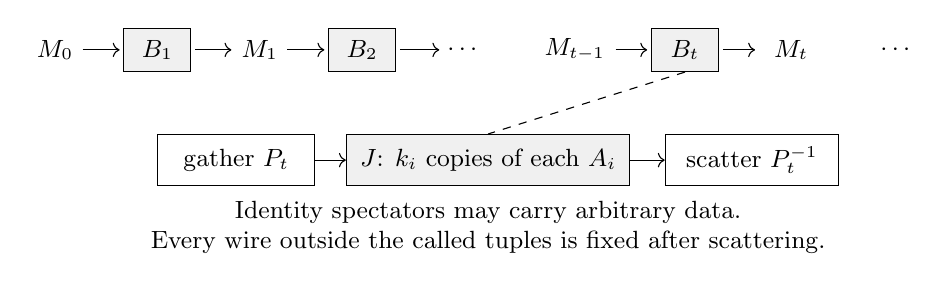
\begin{tikzpicture}[x=1cm,y=1cm, every node/.style={font=\small}]
 \node at (0,1.35) {$M_0$};
 \node[draw,fill=gray!12,minimum width=.85cm,minimum height=.55cm] (b1) at (1.3,1.35) {$B_1$};
 \node at (2.6,1.35) {$M_1$};
 \node[draw,fill=gray!12,minimum width=.85cm,minimum height=.55cm] (b2) at (3.9,1.35) {$B_2$};
 \node at (5.2,1.35) {$\cdots$};
 \node at (6.6,1.35) {$M_{t-1}$};
 \node[draw,fill=gray!12,minimum width=.85cm,minimum height=.55cm] (bt) at (8,1.35) {$B_t$};
 \node at (9.35,1.35) {$M_t$};
 \node at (10.7,1.35) {$\cdots$};
 \draw[->] (.35,1.35)--(.82,1.35);
 \draw[->] (1.78,1.35)--(2.24,1.35);
 \draw[->] (2.95,1.35)--(3.42,1.35);
 \draw[->] (4.38,1.35)--(4.88,1.35);
 \draw[->] (7.12,1.35)--(7.52,1.35);
 \draw[->] (8.48,1.35)--(8.89,1.35);
 \node[draw,minimum width=2cm,minimum height=.65cm] (g) at (2.3,-.05) {gather $P_t$};
 \node[draw,fill=gray!12,minimum width=3.6cm,minimum height=.65cm] (j) at (5.5,-.05) {$J$: $k_i$ copies of each $A_i$};
 \node[draw,minimum width=2.2cm,minimum height=.65cm] (s) at (8.85,-.05) {scatter $P_t^{-1}$};
 \draw[->] (g.east)--(j.west);
 \draw[->] (j.east)--(s.west);
 \draw[dashed] (bt.south)--(j.north);
 \node[align=center] at (5.5,-.9) {Identity spectators may carry arbitrary data.\\
 Every wire outside the called tuples is fixed after scattering.};
\end{tikzpicture}
\caption{Chronological gaps preserve each local word.  Each simultaneous
call slot is one embedded $J$ call with its gather and scatter permutations.}
\label{price:packing-diagram}
\end{figure}

Thus the matrix product
\begin{equation}
 M_TB_TM_{T-1}\cdots M_1B_1M_0
 \label{price:assembled-word}
\end{equation}
restricts to the prescribed program on every active sector and to
identity on every dummy group and unused identity wire.  It is exactly
\(J^{\otimes b}\).  By \cref{price:gather-scatter} it uses precisely
\(T<bw^{b-1}\) calls to \(J\), with all remaining operations monomial,
on precisely \(w^b\) wires.  Since at least one \(A_i\) occurs in
\(J\), the matrix \(J\) is nonmonomial.  This is a finite win,
contrary to the assumption.
\end{proof}

\subsection{Separation, normalization, and compactness}

For a nonempty finite comparison family on a nonempty finite type list,
\cref{price:packing} says that the convex hull of its difference vectors
is disjoint from the open positive orthant \((0,\infty)^m\).
Finite-dimensional separation supplies a nonzero vector \(v\) and a
real number \(c\) with
\[
 v\cdot\Delta^{(r)}\leq c\leq v\cdot y
 \quad\text{for all $r$ and all }y\in(0,\infty)^m;
\]
see \citet[Section~2.5.1, p.~46]{boydVandenberghe2004}.
If a coordinate of \(v\) were negative, sending that coordinate of
\(y\) to infinity would contradict the lower bound by \(c\).
Thus \(v\geq0\).  The infimum of \(v\cdot y\) on the positive
orthant is zero, so \(c\leq0\).  We have obtained nonnegative prices,
not all zero, satisfying every comparison in the finite family.
For an empty family any nonzero nonnegative vector suffices.

We next prevent the normalization from escaping along different types.
Include the fixed shear \(U\) of \cref{price:normalization} in every
finite type list.  For each nonmonomial \(A\) of width \(q\), fix the
following two words once and for all.  Gaussian elimination implements
\(A\) by a finite positive number \(C_A\) of embedded \(U\)-calls
and monomials.  Indeed row permutations and nonzero row scalings are
monomial, and every nonzero row addition is a diagonal conjugate of an
ordered \(U\)-call.  The comparison with one-factor target \(A\)
imposes
\[
 p(A)\leq C_Ap(U).
\]
On width \(2q\), apply \cref{lem:generation} to
\(A\oplus I_q\).  Its calls are embedded calls to \(A\), and it
generates \(U\otimes I_q\) by some fixed word with \(e_A>0\)
such calls and monomials.  The two-factor target \(U\otimes I_q\)
has standard count \(q\) for \(U\), giving
\[
 q p(U)\leq e_Ap(A).
\]
Consequently these two comparisons impose the fixed bounds
\begin{equation}
 c_Ap(U)\leq p(A)\leq C_Ap(U),\qquad c_A=q/e_A>0.
 \label{price:fixed-bounds}
\end{equation}
They introduce no new nonmonomial type other than \(A\) and \(U\).
For \(A=U\), take simply \(c_U=C_U=1\).

Augment any finite comparison family by these bounds for all its types.
Separation gives a nonzero nonnegative solution.  If its \(U\)-price
were zero, every other coordinate would be zero by the upper bounds,
which is impossible.  Divide by its positive \(U\)-price to obtain
\(p(U)=1\).  Applying this argument just to the bounds for one type
also proves that each fixed interval \([c_A,C_A]\) is nonempty.

The collection of all finite complex matrices is a set, as it is
contained in \(\bigcup_{n\geq1}\C^{n^2}\).  Form the product over
all nonmonomial invertible matrices
\[
 \mathcal P=\prod_A[c_A,C_A].
\]
Each factor is a nonempty compact interval, so this product is compact
in the product topology by Tychonov's Theorem
\citep[Tag~08ZU, Theorem~5.14.4]{stacksProject}.
Each comparison specifies a closed subset of \(\mathcal P\), since
it is a linear inequality in finitely many coordinate projections.
Any finite collection of these closed subsets has nonempty intersection:
apply the preceding finite argument to its types, include \(U\), and
augment with their fixed bounds; all other coordinates can be assigned
their lower endpoints.  Compactness gives a point satisfying every
comparison simultaneously.  Call this preliminary function \(p_0\),
and set \(p_0(A)=0\) on monomial matrices.  It is strictly positive
on each nonmonomial matrix, and \(p_0(U)=1\).

\subsection{Algebraic laws and symmetry}

We derive the laws from the comparisons before symmetrizing.  A
one-factor target \(AB\), implemented by consecutive calls to \(B\)
and \(A\), gives
\(p_0(AB)\leq p_0(A)+p_0(B)\).  This remains true if any of the
matrices is monomial, since its call is then a monomial operation of
price zero.  Multiplication by monomials on either side cannot increase
price.  Applying the same observation with their inverses shows
\(p_0(LAR)=p_0(A)\).

The standard axis program for the one-factor target \(A\otimes B\)
gives
\[
 p_0(A\otimes B)\leq |B|p_0(A)+|A|p_0(B).
\]
For the reverse inequality, use the two-factor target \(A\otimes B\)
and the word consisting of one call to that entire matrix.  Its
comparison gives the opposite inequality.  Hence the tensor law is
exact, including when a factor is an identity or any other monomial.

For direct sums the one-factor target \(A\oplus B\), implemented
by disjoint calls to its two blocks, gives
\(p_0(A\oplus B)\leq p_0(A)+p_0(B)\).  The reverse inequality
requires a separate construction.  Put \(a=|A|\), \(e=|B|\), and
\[
 X=A^{\otimes a}\otimes B^{\otimes e},\qquad Q=|X|.
\]
Consider the tensor target \(X\otimes I_2\), with its factors listed
as \(a\) copies of \(A\), \(e\) copies of \(B\), and \(I_2\).
After a coordinate permutation this is two independent copies of \(X\); this statement
is an identity of matrices and does not use a direct-sum price law.
In the first copy run all \(A\)-axes and then all \(B\)-axes.
In the second copy run all \(B\)-axes and then all \(A\)-axes.
There are exactly \(aQ/a=Q\) individual \(A\)-calls and
\(eQ/e=Q\) individual \(B\)-calls in each copy.
Pair the successive \(Q\) first-stage \(A\)-calls of the first
copy with the successive \(Q\) first-stage \(B\)-calls of the
second copy.  Each pair acts on disjoint tuples and is one embedded
\(A\oplus B\)-call, after gathering its coordinates.  Pair the
second stages in the same manner, reversing which copy supplies which
type.  Each copy retains its own required call order.  We obtain a word
with \(2Q\) calls to \(A\oplus B\), with only permutations added.
The comparison for the displayed tensor target therefore gives
\[
 2Q\bigl(p_0(A)+p_0(B)\bigr)
       \leq2Qp_0(A\oplus B).
\]
The construction also applies when one or both factors are monomial:
we may keep their individual block operations in the pairing, while
their contribution to the comparison is zero.  Thus direct-sum
additivity is established without using it to produce the two copies.

Finally define
\begin{equation}
 p(A)=\tfrac14\bigl(p_0(A)+p_0(A^{-1})
                 +p_0(A^{\mathsf T})+p_0(A^{-\mathsf T})\bigr).
 \label{price:averaging}
\end{equation}
Inversion and transposition commute and each has order two, so this
function has both symmetries.  Each of the four summands retains product
subadditivity: transposition or inversion may reverse the order of
\(AB\), but the scalar upper bound is still \(p_0(A)+p_0(B)\)
with the corresponding transforms.  They retain both exact laws because
inverse and transpose act componentwise on tensor products and direct
sums.  They retain monomial invariance, and are positive exactly on
nonmonomials, because these operations preserve the class of monomial
matrices.  Also \(U^{-1}\) is conjugate to \(U\) by
\(\diag(1,-1)\), and \(U^{\mathsf T}\) is conjugate to \(U\)
by the two-coordinate swap.  Thus every summand in
\cref{price:averaging} has value one at \(U\).  This proves
\cref{thm:prices}.  All subsequent arguments use this symmetric \(p\)
and its proved laws, without imposing additional comparison constraints
on the average.

\begin{corollary}[Shears, pairs, and embedded words]
\label{price:word-bounds}
Every nontrivial elementary coordinate shear has price one, including
with any number of untouched coordinates.  Every invertible
\(2\times2\) matrix has price at most two.  If a word on \(w\)
coordinates implements \(G\), using nonmonomial calls
\(A_1,\ldots,A_l\) and monomials, then
\[
 p(G)\leq\sum_{j=1}^l p(A_j).
\]
If the word instead implements \(G\oplus I_s\), the same bound holds
for \(p(G)\), with no restriction on the initial values of the
\(s\) coordinates restored by the word.
\end{corollary}

\begin{proof}
A shear adding a nonzero multiple of one coordinate into another is a
monomial conjugate of \(U\oplus I\), so its price is one by
\cref{price:monomial-law,price:sum-law,price:normalization}.
For an invertible pair matrix, first permute rows if needed to make its
upper-left entry nonzero.  With entries \(\alpha,\beta,\gamma,\delta\)
and determinant \(D\ne0\), it factors as
\[
 \begin{pmatrix}\alpha&\beta\\\gamma&\delta\end{pmatrix}
 =\begin{pmatrix}1&0\\\gamma/\alpha&1\end{pmatrix}
  \begin{pmatrix}\alpha&0\\0&D/\alpha\end{pmatrix}
  \begin{pmatrix}1&\beta/\alpha\\0&1\end{pmatrix}.
\]
This uses at most two nontrivial shears and a monomial.  Finally an
embedded call to \(A\) is a permutation conjugate of
\(A\oplus I_{w-|A|}\), omitting the identity block when it has size
zero, whose price is \(p(A)\).  Repeated product
subadditivity gives the word bound.  Identity padding has price zero
by direct-sum additivity.  The last assertion is an exact matrix
identity on all input coordinates; it does not assume zero scratch
values.
\end{proof}

\section{Triangular matrices and invertible corners}
\label{corner:sec:corners}

Continue under the no-finite-win assumption and fix the symmetric price
of \cref{thm:prices}. Our goal is contraction to an invertible submatrix.

\begin{theorem}[Invertible corners]
\label{thm:corner}
If an invertible matrix $K$ has an invertible square submatrix $M$,
then $p(M)\le p(K)$.
\end{theorem}

Independent row and column permutations move $M$ to a corner without
changing the price of $K$. To compare their prices, we will run the
resulting block matrix along many tensor axes and for many time steps.
The other coordinates persist as state between successive steps. Their
initial values affect the output, so the main task is to remove that
contribution at a cost small compared with the number of calls.

We first obtain price bounds for rectangular shears and scalar
convolutions. We then prove that a block triangular matrix costs at
least the sum of its diagonal blocks. These tools allow us to correct
the initial state in a long cascade and isolate the repeated tensor
powers of $M$ that prove the theorem. The one-way price bound for a scalar circuit
is a consequence of the corner theorem, derived at the end of the
section; the preliminary convolution estimate uses circuits in both
directions.

\subsection{Rectangular shears and scalar convolution}

For $G\in\Mat_{a\times b}(\C)$ put
\[
 s(G)=p\left(\begin{pmatrix}I_a&G\\0&I_b\end{pmatrix}\right).
\]
Its action on $(y,x)$ is $(y+Gx,x)$.  Empty blocks can be omitted.

\begin{lemma}[A rectangular shear from a linear DAG]
\label{lem:shear-dag}
Suppose a permitted linear DAG with $l$ scalar gates computes $Gx$,
with $a$ designated output coordinates.  Then
\begin{equation}
 s(G)\le 8l+2a.
 \label{corner:eq:shear-dag}
\end{equation}
If only $a_0$ rows of $G$ are nonzero, $a$ may be replaced by $a_0$.
The constant is independent of the dimensions and all circuit scalars.
\end{lemma}

\begin{proof}
A finite DAG has finite depth and finite maximum fan-out, counting
repeated operand edges and designated output uses.  Apply
\cref{fft:dirty-layers} to this DAG with source coordinates $x$,
target coordinates $y$, and one additional coordinate per gate,
with arbitrary initial values.  It gives at most $8l+2a$ elementary
shears realizing $(x,y,z)\mapsto(x,y+Gx,z)$.
Although depth and fan-out may vary with the DAG, the shear count is
independent of both; the layer bound is not needed here.
By \cref{price:word-bounds} and identity padding, this proves
\cref{corner:eq:shear-dag}.  If only $a_0$ rows are nonzero, apply the
same replay to the submap of those rows, retaining all $l$ gate
coordinates, and identity-pad the omitted targets.  This gives
$8l+2a_0$ instead; if $a_0=0$, the shear is identity.
\end{proof}

For an invertible $m\times m$ matrix $G$, the exact identity
\begin{equation}
 \begin{pmatrix}I&G\\0&I\end{pmatrix}
 \begin{pmatrix}I&0\\-G^{-1}&I\end{pmatrix}
 \begin{pmatrix}I&G\\0&I\end{pmatrix}
 =\begin{pmatrix}0&G\\-G^{-1}&0\end{pmatrix}
 \label{corner:eq:two-way-identity}
\end{equation}
gives
\begin{equation}
 2p(G)\le 2s(G)+s(G^{-1}).
 \label{corner:eq:two-way-bound}
\end{equation}
Indeed the right side of \cref{corner:eq:two-way-identity} is
monomial-equivalent to $G\oplus G^{-1}$, while exchanging the two
coordinate groups and changing signs identifies the middle shear's
price with $s(G^{-1})$.  Consequently circuits for both $G$ and
$G^{-1}$, of sizes $l$ and $l'$, give
$p(G)=O(l+l'+m)$ with a universal constant.

For a scalar or matrix formal power series $F(z)$, let
$\mathcal T_t(F)$ be multiplication by $F(z)$ modulo $z^t$, in the
coefficient basis ordered with time first.  Thus, if
$F(z)=\sum_{j\ge0}F_jz^j$, its $(a,b)$ block is $F_{a-b}$ for
$0\le b\le a<t$, and is zero otherwise.  Coefficients with negative
indices mean zero.  Series multiplication gives
\begin{equation}
 \mathcal T_t(FG)=\mathcal T_t(F)\mathcal T_t(G).
 \label{corner:eq:truncation-product}
\end{equation}
In particular, invertibility of $F_0$ implies invertibility of
$\mathcal T_t(F)$, with inverse $\mathcal T_t(F^{-1})$.

\begin{lemma}[Scalar convolution]
\label{lem:scalar-convolution}
For every scalar formal series $f$ with $f(0)\ne0$ and every $t\ge1$,
\[
 p(\mathcal T_t(f))=O(t\log(2t)),
\]
with an absolute implied constant, independent of the coefficients of
$f$ and of their possible dependence on $t$.
\end{lemma}

\begin{proof}
Only the first $t$ coefficients of $f$ affect the matrix.  Pad these
coefficients and the input coefficient vector to a power-of-two length
$m$ with $2t\le m<4t$.  A length-$m$ Fourier transform, multiplication
by the prechosen Fourier transform of the fixed kernel, and an inverse
Fourier transform compute their ordinary convolution, since its degree
is at most $2t-2<m$.  Selecting the first $t$ coefficients gives
$\mathcal T_t(f)$.  The binary Fourier recursion splits even and odd
indices and combines each pair by one scalar multiplication and two
additions or subtractions, so it and its inverse use
$O(m\log(2m))$ permitted scalar gates.  The frequency scalings and
inverse normalization cost $O(m)$ gates, even when some kernel
frequencies are zero.  This is a DAG construction and does not require
those intermediate scalings to be invertible.

Exactly the same construction applies to the first $t$ coefficients
of $1/f$, which exist because $f(0)\ne0$.  Apply
\cref{lem:shear-dag,corner:eq:two-way-bound} to these two DAGs.
Every kernel coefficient and Fourier constant is prechosen; there is
no charge for generating its description, but its multiplication on
variable data has been included in the count.
\end{proof}

\subsection{Triangular monotonicity by whole-block compression}

\begin{lemma}[Triangular monotonicity]
\label{lem:triangular}
If $M\in\GL_n(\C)$, $D\in\GL_r(\C)$ and
$C\in\Mat_{n\times r}(\C)$, then
\begin{equation}
 p\left(\begin{pmatrix}M&C\\0&D\end{pmatrix}\right)
 \ge p(M)+p(D).
 \label{corner:eq:triangular}
\end{equation}
The same conclusion holds for the lower triangular orientation, and
the price of any invertible block triangular matrix is at least the
sum of the prices of its invertible diagonal blocks.
\end{lemma}

\begin{proof}
Write $K=\begin{pmatrix}M&C\\0&D\end{pmatrix}$ and fix $k\ge1$.
The usual computation of $Y=D^{\otimes k}$ on $R=r^k$ bottom
coordinates applies $D$ along axes $1,\ldots,k$, using
$u=kr^{k-1}$ calls.  Replace each call by a $K$ call, supplying a
fresh group of $n$ data coordinates for its $M$ side.  Since these
groups are used only once and do not affect the bottom coordinates,
the resulting matrix is
\[
 \begin{pmatrix}I_u\otimes M&E\\0&Y\end{pmatrix},
 \qquad p\left(\begin{pmatrix}I_u\otimes M&E\\0&Y\end{pmatrix}\right)
 \le u p(K).
\]
We will compress the $u$ whole $n\times R$ row blocks of $EY^{-1}$.
No independent change of its individual scalar rows is used.

Label a call by its axis $j$ and fiber indices
$\mathbf i=(i_\ell)_{\ell\ne j}$.  For $1\le a\le n$ and a bottom
multi-index $\boldsymbol\ell=(\ell_1,\ldots,\ell_k)$, its row block
$R_{j,\mathbf i}$ in $EY^{-1}$ has entries
\begin{equation}
 (R_{j,\mathbf i})_{a,\boldsymbol\ell}
 =(CD^{-1})_{a,\ell_j}
   \prod_{h<j}\delta_{i_h,\ell_h}
   \prod_{h>j}(D^{-1})_{i_h,\ell_h}.
 \label{corner:eq:actual-row-block}
\end{equation}
To see this, the call's contamination uses $C$ at axis $j$, with
$D$ already applied on axes $h<j$ and identity on axes $h>j$.
Multiplication by $Y^{-1}$ cancels the earlier $D$ factors, leaves
$CD^{-1}$ locally, and introduces $D^{-1}$ on the later axes.

For fixed $j$, insertion of the fixed matrix $CD^{-1}$ in the $j$th
slot defines a linear map from the complementary tensor covector
space to $\Mat_{n\times R}(\C)$.  The complementary covectors in
\cref{corner:eq:actual-row-block} form a basis, because every
$D^{-1}$ is invertible.  Coordinate covectors form another basis.
The images of either basis therefore span the same image space,
whether or not this linear map is injective.  Images of coordinate
covectors have at most $nr$ nonzero entries.  Taking their union over
$j$ gives a sparse spanning family for the span $S$ of all actual
row blocks.  Select a basis $B_1,\ldots,B_h$ from this family; then
\[
 h\le\min(u,nR),\qquad \nnz(B_i)\le nr.
\]
Overlaps between axis spans and dependencies among rows of $C$ can
only decrease $h$.

The map $\Phi:\C^u\longrightarrow S$ sending coefficients to their
linear combination of the actual row blocks is surjective.  Choose
one lift of each $B_i$ under $\Phi$, and append a basis of
$\ker\Phi$.  These $u$ vectors form a basis of $\C^u$: applying
$\Phi$ to a relation first kills the coefficients of the $B_i$, and
then independence in the kernel kills the others.  Put these vectors
as the rows of $V\in\GL_u(\C)$.  Postapply $V\otimes I_n$ to the
data groups.  The data block becomes exactly
\[
 (V\otimes I_n)(I_u\otimes M)=V\otimes M,
\]
while its contamination expressed in the final bottom variables is
the stack $B_1,\ldots,B_h,0,\ldots,0$.  Cancel it by at most $hnr$
elementary shears from those bottom variables into the data groups.
The final map is exactly $(V\otimes M)\oplus Y$.

The previously proved price laws now give
\[
 n p(V)+u p(M)+u p(D)
 \le u p(K)+n p(V)+hnr.
\]
The identical $n p(V)$ terms cancel, without any estimate on $V$.
Since $h\le nr^k$, division by $u=kr^{k-1}$ yields
\[
 p(M)+p(D)\le p(K)+\frac{n^2r^2}{k}.
\]
Let $k$ tend to infinity with $K,n,r$ fixed.  This proves
\cref{corner:eq:triangular}.  If $r=1$, the same construction has
$R=1$, $u=k$ and error at most $n^2/k$.  If $S=0$, there are no
$B_i$ and a kernel basis alone supplies $V$; no cancellation shears
are needed.  Empty diagonal blocks simply reduce to the other block.
Exchanging the two groups proves the lower triangular case, and
induction on the number of blocks proves the last assertion.
\end{proof}

\subsection{A time cascade and its initial-state correction}

Fix an invertible cell
\begin{equation}
 K=\begin{pmatrix}M&C\\B&D\end{pmatrix},\qquad
 M\in\GL_n(\C),\quad D\in\Mat_{r\times r}(\C),
 \qquad H(z)=M+zC(I_r-zD)^{-1}B.
 \label{corner:eq:cell}
\end{equation}
No invertibility of $D$ is required.  The transfer matrix $H$ is
regular at zero and $H(0)=M$.  For one fiber, with incoming state
$w_\tau$, input $x_\tau$ and output $y_\tau$, the cell equations are
\[
 y_\tau=Mx_\tau+Cw_\tau,\qquad
 w_{\tau+1}=Bx_\tau+Dw_\tau.
\]
Writing series in time and retaining coefficients below $t$ gives
\[
 w(z)=w_0+zBx(z)+zDw(z),\qquad
 y(z)=H(z)x(z)+C(I_r-zD)^{-1}w_0 \pmod {z^t}.
\]
These are identities between finite coefficient maps, rather than
operations that a circuit is asked to perform implicitly.

For $k\ge1$ put $N=n^k$.  At each tick, apply the cell along each of
the $k$ spatial tensor axes in order, using $n^{k-1}$ disjoint fibers
per axis.  Axis $j$ has its own persistent state space
\[
 W_j=(\C^n)^{\otimes(j-1)}\otimes\C^r
             \otimes(\C^n)^{\otimes(k-j)}.
\]
States of different axes are distinct, and each $W_j$ is carried
from one tick to the next.  The $t$ data blocks are fresh inputs,
one per tick.  The entire computation is a word in invertible $K$
calls on $tN+krn^{k-1}$ coordinates; denote its matrix by
$\mathcal K_{k,t}$.  \Cref{corner:fig:cascade} shows two successive
ticks and the distinct state spaces carried by the axes from one tick
to the next.

\begin{figure}[ht]
\centering
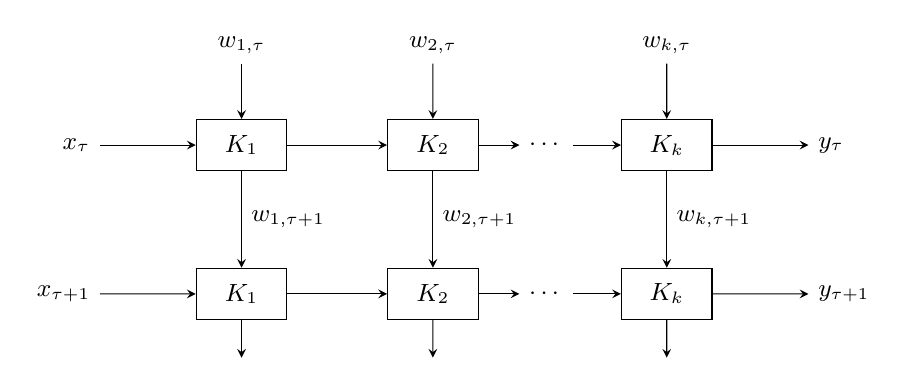
\begin{tikzpicture}[>=stealth,scale=.9,every node/.style={font=\small}]
 \node[draw,minimum width=1.15cm,minimum height=.65cm] (a1) at (0,0) {$K_1$};
 \node[draw,minimum width=1.15cm,minimum height=.65cm] (a2) at (2.7,0) {$K_2$};
 \node (ad) at (4.3,0) {$\cdots$};
 \node[draw,minimum width=1.15cm,minimum height=.65cm] (ak) at (6,0) {$K_k$};
 \node[draw,minimum width=1.15cm,minimum height=.65cm] (b1) at (0,-2.1) {$K_1$};
 \node[draw,minimum width=1.15cm,minimum height=.65cm] (b2) at (2.7,-2.1) {$K_2$};
 \node (bd) at (4.3,-2.1) {$\cdots$};
 \node[draw,minimum width=1.15cm,minimum height=.65cm] (bk) at (6,-2.1) {$K_k$};
 \draw[->] (-2,0) node[left] {$x_\tau$} -- (a1);
 \draw[->] (a1) -- (a2);
 \draw[->] (a2) -- (ad);
 \draw[->] (ad) -- (ak);
 \draw[->] (ak) -- (8,0) node[right] {$y_\tau$};
 \draw[->] (-2,-2.1) node[left] {$x_{\tau+1}$} -- (b1);
 \draw[->] (b1) -- (b2);
 \draw[->] (b2) -- (bd);
 \draw[->] (bd) -- (bk);
 \draw[->] (bk) -- (8,-2.1) node[right] {$y_{\tau+1}$};
 \draw[->] (0,1.15) node[above] {$w_{1,\tau}$} -- (a1.north);
 \draw[->] (2.7,1.15) node[above] {$w_{2,\tau}$} -- (a2.north);
 \draw[->] (6,1.15) node[above] {$w_{k,\tau}$} -- (ak.north);
 \draw[->] (a1.south) -- node[right] {$w_{1,\tau+1}$} (b1.north);
 \draw[->] (a2.south) -- node[right] {$w_{2,\tau+1}$} (b2.north);
 \draw[->] (ak.south) -- node[right] {$w_{k,\tau+1}$} (bk.north);
 \draw[->] (b1.south) -- (0,-3);
 \draw[->] (b2.south) -- (2.7,-3);
 \draw[->] (bk.south) -- (6,-3);
\end{tikzpicture}
\caption{Two ticks of the cascade.  Each $K_j$ represents
$n^{k-1}$ disjoint calls along axis $j$.  Horizontal arrows carry
$N$ data coordinates; the separate vertical arrows carry each
axis's $rn^{k-1}$ persistent state coordinates.}
\label{corner:fig:cascade}
\end{figure}

With data coordinates listed before all state coordinates, the
top-left block of $\mathcal K_{k,t}$ is
\[
 A_{k,t}=\mathcal T_t(H_k),\qquad H_k(z)=H(z)^{\otimes k}.
\]
Indeed the direct series response composes the lifts of $H$ on all
axes.  The top-right block $E_t$ consists of the first $t$ coefficients
of $E(z)=[E_1(z)\ \cdots\ E_k(z)]$, where
\begin{equation}
 E_j(z)=I_n^{\otimes(j-1)}\otimes
        \bigl(C(I_r-zD)^{-1}\bigr)\otimes H(z)^{\otimes(k-j)}.
 \label{corner:eq:state-response}
\end{equation}
An initial state at axis $j$ passes through that axis's state-to-data
map and then through the later axes; the earlier axes do not act on
this contribution.  This proves \cref{corner:eq:state-response} as
well as the direct response, including the order of all factors.

\begin{lemma}[Uniform cascade estimate]
\label{corner:lem:cascade}
For each fixed cell $K$ as in \cref{corner:eq:cell}, there is a constant $C_K$
such that, for every $k,t\ge1$ and $N=n^k$,
\begin{equation}
 p\bigl(\mathcal T_t(H^{\otimes k})\bigr)
 \le tk n^{k-1}p(K)
       +C_K\bigl(Nt\log(2t)+(k+1)^3N\bigr).
 \label{corner:eq:cascade-bound}
\end{equation}
The constant is independent of $t$, $k$, and any scalars used for
coefficient interpolation.
\end{lemma}

\begin{proof}
If $r=0$, the state is absent and $H=M=K$ is constant.  The exact
tensor and direct-sum laws already give the assertion.  Suppose
$r\ge1$ and introduce polynomial matrices and scalar polynomials
\[
 \begin{gathered}
 a(z)=\det(I_r-zD),\qquad R(z)=\operatorname{adj}(I_r-zD),\\
 F(z)=a(z)M+zCR(z)B,\qquad
 b(z)=\det F(z),\qquad J(z)=\operatorname{adj}F(z).
 \end{gathered}
\]
Then $H=F/a$, $H^{-1}=aJ/b$, $a(0)=1$, and
$b(0)=\det M\ne0$.  We have
\[
 \deg a\le r,\quad\deg R\le r-1,\quad
 \deg F\le r,\quad\deg b\le nr,\quad\deg J\le(n-1)r.
\]
For $n=1$ the adjugate $J$ is the constant $1$, as required by
these formulas.  Cancelling the later-axis responses in
\cref{corner:eq:state-response} gives
\[
 H_k^{-1}E_j
 =(H^{-1})^{\otimes(j-1)}\otimes(JCR/b)
                         \otimes I_n^{\otimes(k-j)}.
\]
Thus $q_k=b^k$ clears the entire matrix $H_k^{-1}E$.  Its $j$th
cleared block is the following explicit polynomial map $W_j\to\C^N$:
\begin{equation}
 Q_{k,j}(z)
 =a(z)^{j-1}b(z)^{k-j}\Bigl(
    J(z)^{\otimes(j-1)}\otimes\bigl(J(z)CR(z)\bigr)
                     \otimes I_n^{\otimes(k-j)}\Bigr).
 \label{corner:eq:cleared-state}
\end{equation}
Its degree is at most
\[
 (j-1)r+(k-j)nr+(j-1)(n-1)r+(nr-1)=knr-1.
\]
The scalar $q_k$ has degree at most $knr$ and has nonzero constant
term.  The identities also hold when any of the displayed matrix
polynomials vanish.

Here is an explicit DAG bound for the nonzero time coordinates of
$Q_k(z)w=\sum_{j=1}^kQ_{k,j}(z)w_j$.  Put $m=knr$, and choose $m$
distinct complex evaluation points.  Because
\cref{corner:eq:cleared-state} is polynomial, no avoidance of poles
is needed.  At one evaluation point, a rectangular application of
$JCR$ on its $r$-axis costs at most $2rN$ scalar gates.  Applying
$J$ on the preceding $j-1$ axes costs at most $2n(j-1)N$ gates,
by doing the fixed $n\times n$ map on all fibers of each axis.
The scalar factor costs at most $N$ gates.  Adding the $k$
contributions costs at most $(k-1)N$ more.  One evaluation therefore
uses at most
\[
 \bigl(nk(k-1)+2(r+1)k-1\bigr)N=O_K(k^2N)
\]
gates.  All local entries and scalar powers here are prechosen
constants.  Applying the inverse scalar Vandermonde matrix to the
$m$ evaluations, separately on each of the $N$ coordinates, recovers
all $m$ coefficient vectors using at most $2m^2N$ further scalar
gates.  The total is $O_K((k+1)^3N)$.
For any run length $t$, keep only the first $\min(t,m)$ coefficient
vectors; all other rows of the truncated response are zero.  This
bound is consequently uniform in $t$.

Set $P=\mathcal T_t(1/q_k)$ and
$A'=A_{k,t}(P\otimes I_N)$.  In formal series modulo $z^t$,
$A'^{-1}E_t$ is precisely the coefficient map of
$q_kH_k^{-1}E=Q_k$ just constructed.  Hence
\cref{lem:shear-dag}, with zero output rows omitted, bounds the
price of the shear with block $-A'^{-1}E_t$ by
$O_K((k+1)^3N)$.  This uses only the rectangular shear law, not a
price bound for an arbitrary invertible circuit output.

Now form the exact product
\begin{equation}
 \mathcal K_{k,t}
 \begin{pmatrix}P\otimes I_N&0\\0&I\end{pmatrix}
 \begin{pmatrix}I&-A'^{-1}E_t\\0&I\end{pmatrix}.
 \label{corner:eq:state-elimination}
\end{equation}
Its top row of blocks is $(A',0)$.  Each factor is invertible, and
$A'$ is invertible because $H(0)=M$ and $q_k(0)\ne0$.  Therefore
the other diagonal block of this lower triangular product is also
invertible.  By \cref{lem:triangular} its price is at least $p(A')$.
There are $tkn^{k-1}$ cell calls in $\mathcal K_{k,t}$, so
\[
 p(A')\le tkn^{k-1}p(K)+N p(P)+O_K((k+1)^3N).
\]
Here the tensor and direct-sum laws price the scalar preprocessing
by $Np(P)$, including its identity on the state.  Finally
$A_{k,t}=A'(P^{-1}\otimes I_N)$ and inverse symmetry give
\[
 p(A_{k,t})\le tkn^{k-1}p(K)+2Np(P)+O_K((k+1)^3N).
\]
Apply \cref{lem:scalar-convolution} to $P$.  Its bound is uniform
even though $q_k$ varies with $k$, proving
\cref{corner:eq:cascade-bound}.
\end{proof}

\subsection{Proof of the corner law and its circuit consequence}

\begin{proof}[Proof of \cref{thm:corner}]
Independent row and column permutations move $M$ to the top-left
corner and preserve $p(K)$.  Write the resulting matrix as in
\cref{corner:eq:cell}.  If the complementary width is zero the claim
is equality; otherwise apply \cref{corner:lem:cascade}.  The matrix
$A_{k,t}=\mathcal T_t(H^{\otimes k})$ is lower triangular in time
with $t$ identical diagonal blocks $M^{\otimes k}$.  Thus
\cref{lem:triangular} and the tensor law imply
\[
 p(A_{k,t})\ge t p(M^{\otimes k})
             =tkn^{k-1}p(M).
\]
Fix $K,n,r$ first and use the bound of
\cref{corner:eq:cascade-bound}.  For example, choose
$t=t(k)=2^{\lceil8\log_2(k+1)\rceil}$, so
$(k+1)^8\le t<2(k+1)^8$.  Division by $tkn^{k-1}=tkN/n$ gives
\[
 p(M)\le p(K)+C_K n\left(
       \frac{\log(2t)}{k}+\frac{(k+1)^3}{tk}\right).
\]
Both errors tend to zero.  The matrices $M$ and $K$ in this real
inequality are fixed, so it proves the exact inequality
$p(M)\le p(K)$.  No continuity assertion about the price, or
limiting circuit for a matrix, has been used.  A zero-size submatrix,
if allowed, can simply be omitted and assigned price zero.
\end{proof}

\begin{corollary}[A universal one-way DAG price bound]
\label{cor:dag-price}
If $G\in\GL_m(\C)$ has a permitted linear DAG with $l$ scalar
gates, then
\[
 p(G)\le s(G)\le 8l+2m.
\]
The bound holds with the same constants for all dimensions and all
matrix families, without requiring a DAG for $G^{-1}$.
\end{corollary}

\begin{proof}
$G$ is an invertible square submatrix of
$\begin{pmatrix}I_m&G\\0&I_m\end{pmatrix}$, so
\cref{thm:corner} gives its first inequality, and
\cref{lem:shear-dag} gives the second.  Although the proof of the
corner law fixed each individual matrix while taking a limit, the
resulting inequality is exact for every finite matrix.  The numerical
constants here come entirely from the dirty scratch simulation.
\end{proof}

\section{Changing the coefficient boundary and specializing prices}
\label{feedback:sec}

The corner law compares the price of an invertible matrix with that
of an invertible submatrix. We now consider a different operation on
the cell from the preceding section. Write
\[
 K=\begin{pmatrix}M&C\\B&D\end{pmatrix}\in\GL_{n+r}(\C),\qquad
 K(x,w)=(y,w'),\qquad M\in\GL_n(\C).
\]
Closing its state connection at a scalar $s$ means imposing $w=sw'$.
When $I_r-sD$ is invertible, the state equation gives
\[
 w=s(I_r-sD)^{-1}Bx,\qquad
 y=H(s)x,\qquad H(z)=M+zC(I_r-zD)^{-1}B.
\]
Our first objective is to prove $p(H(s))\le p(K)$ whenever $H(s)$
is invertible. We will then prove that a uniform
price bound for a rational matrix at generic scalar values remains
valid at every regular invertible value. Closing the connection serves
only to define the finite matrix $H(s)$; every price inequality concerns
ordinary invertible matrices.

Both arguments use a common comparison between coefficient boundary
conditions. The data-to-data block of the preceding cascade is multiplication
by a matrix series modulo $z^t$. We compare this with multiplication
modulo a different scalar polynomial of degree $t$. For a $k$th tensor
power, a scalar change of coordinates confines the discrepancy to
$O(k)$ time indices. We must also control the large spatial matrix on
those indices: an explicit common family of inexpensive generators
supplies this second bound. The resulting estimate is uniform over the
scalar modulus, which can therefore be chosen separately at each tensor
order.

We retain the time coefficient convention for $\mathcal T_t$: for a
matrix series $F(z)$ regular at zero, $\mathcal T_t(F)$ sends the
coefficients of $x(z)$, of degree less than $t$, to those of $F(z)x(z)$
modulo $z^t$, with the time index outermost. All prices in this section
satisfy the laws of \cref{thm:prices}.

\subsection{A uniform comparison for scalar moduli}

\begin{lemma}[Coefficient-boundary comparison]
\label{lem:boundary-comparison}
Fix $G(z)\in\Mat_n(\C[z])$ with $G(0)$ invertible.  There is a constant
$C_G$ with the following property.  Let $k\geq1$, put $N=n^k$ and
$d=k\deg G$, and let $t>d$ be an integer.  Suppose $\ell(z)$ is monic of
degree $t$, $\ell(0)\ne0$, and multiplication by $G(z)^{\otimes k}$ on
$(\C[z]/(\ell))^N$ is invertible.  Denote its matrix in the coefficient
basis by $W$, and put
\[
 A_G=\mathcal T_t(G(z)^{\otimes k}).
\]
Then
\begin{equation}
 \bigl|p(W)-p(A_G)\bigr|
 \leq C_G N\bigl(t\log(2t)+(k+1)^6\bigr).
 \label{feedback:eq:boundary-error}
\end{equation}
The constant is independent of $k,t,\ell$ and of the magnitudes of the
coefficients of $\ell$.  In particular, for
\begin{equation}
 t=t(k)=2^{\lceil 8\log_2(k+1)\rceil},
 \qquad (k+1)^8\leq t<2(k+1)^8,
 \label{feedback:eq:common-length}
\end{equation}
the difference is $o(tkN)$, uniformly over every admissible modulus of
that degree.
\end{lemma}

\begin{proof}
Choose once and for all polynomial $J(z)$ and scalar polynomial $u(z)$
such that
\[
 G(z)^{-1}=J(z)/u(z),\qquad u(0)\ne0;
\]
for example, take $J=\operatorname{adj}G$ and $u=\det G$.  Write
\[
 G_k(z)=G(z)^{\otimes k}=\sum_{j=0}^{d}G_jz^j,
 \qquad
 J_k(z)=J(z)^{\otimes k}=\sum_{i=0}^{e}J_iz^i,
 \qquad e=k\deg J.
\]
These are degree bounds with zero coefficient matrices permitted.
The subscript on $G_j$ or $J_i$ in this proof denotes a coefficient of
the tensor power, rather than of the original fixed matrix.
Both $d$ and $e$ are bounded by a fixed multiple of $k$.
If $d=0$, multiplication is coefficientwise, so $W=A_G$ and the result
holds.  Assume $d>0$ and set $T=t-d$.

Let $L=W-A_G$.  An input supported at times less than $T$ has product
with $G_k$ of degree less than $t$, so $L$ has zero columns at those
times.  Scalar polynomial division also shows that, for every input
$x(z)$ of degree less than $t$,
\begin{equation}
 Lx=\ell(z)v_x(z)\pmod {z^t},\qquad \deg v_x<d.
 \label{feedback:eq:boundary-quotient}
\end{equation}
Here $v_x$ is minus the quotient of $G_kx$ by $\ell$, with scalar
division applied to every coordinate.  The degree bound follows from
$\deg(G_kx)<t+d$.

The invertible relative map and the scalar prefix map are
\[
 R=A_G^{-1}W=I+S,\qquad S=A_G^{-1}L,
 \qquad
 P=\mathcal T_T(u^k/\ell)\oplus I_d.
\]
The series in $P$ is regular and nonzero at zero.  Since $S$ has zero
prefix columns and $P^{-1}$ is identity on the suffix of length $d$,
\begin{equation}
 S(P^{-1}\otimes I_N)=S,\qquad
 \widehat R=(P\otimes I_N)R(P^{-1}\otimes I_N)
           =I+(P\otimes I_N)S.
 \label{feedback:eq:prefix-conjugation}
\end{equation}
This identity uses the entire prefix--suffix decomposition; a general
scalar change of basis on all $t$ times would not have this property.

On the prefix, the output of the correction in
\cref{feedback:eq:prefix-conjugation} is, modulo $z^T$,
\[
 \frac{u^k}{\ell}\frac{J_k}{u^k}\ell v_x=J_kv_x.
\]
It therefore vanishes at prefix times greater than or equal to $e+d$.
Define the disjoint sets
\[
 \mathcal E=\{0,\ldots,\min(T,e+d)-1\},\quad
 \mathcal B=\{T,\ldots,t-1\},\quad
 \mathcal U=\mathcal E\cup\mathcal B.
\]
The correction has columns only in $\mathcal B$ and rows only in
$\mathcal U$, where $|\mathcal U|\leq e+2d=O(k)$.
Thus both blocks coupling $\mathcal U$ to its complement are zero in
the correction.  A simultaneous permutation of rows and columns gives
\begin{equation}
 \widehat R\simeq R_{\mathcal U}\oplus
 I_{(t-|\mathcal U|)N},
 \qquad R_{\mathcal U}\in\GL_{|\mathcal U|N}(\C).
 \label{feedback:eq:active-summand}
\end{equation}
Invertibility of the active block follows from invertibility of
$\widehat R$.  If the coarse early and suffix ranges would overlap,
the minimum in $\mathcal E$ truncates the former: the middle set is
then empty and $t\leq e+2d$.  The bound and the direct-sum conclusion
still hold.  \Cref{feedback:fig:boundary-support} displays the support
of the correction $\widehat R-I$ when the middle set is nonempty.

\begin{figure}[t]
\centering
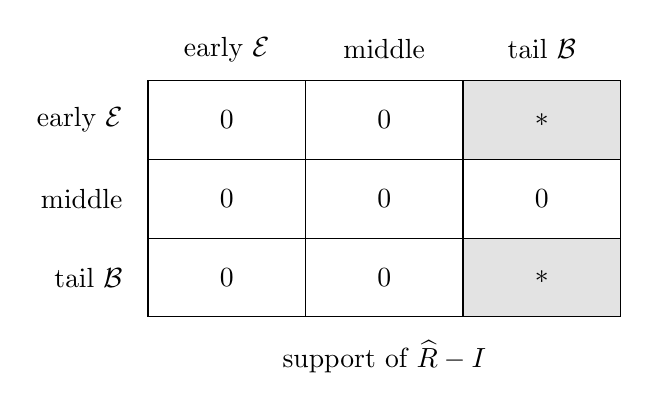
\begin{tikzpicture}[x=1cm,y=1cm]
 \fill[gray!22] (4,2) rectangle (6,3);
 \fill[gray!22] (4,0) rectangle (6,1);
 \draw (0,0) rectangle (6,3);
 \draw (2,0)--(2,3) (4,0)--(4,3);
 \draw (0,1)--(6,1) (0,2)--(6,2);
 \node at (1,3.4) {early $\mathcal E$};
 \node at (3,3.4) {middle};
 \node at (5,3.4) {tail $\mathcal B$};
 \node[anchor=east] at (-.2,2.5) {early $\mathcal E$};
 \node[anchor=east] at (-.2,1.5) {middle};
 \node[anchor=east] at (-.2,.5) {tail $\mathcal B$};
 \foreach \x/\y in {1/.5,1/1.5,1/2.5,3/.5,3/1.5,3/2.5,5/1.5}
   \node at (\x,\y) {$0$};
 \node at (5,2.5) {$*$};
 \node at (5,.5) {$*$};
 \node at (3,-.5) {support of $\widehat R-I$};
\end{tikzpicture}
\caption{After prefix conjugation, only the shaded blocks can be
nonzero in the correction.  Restoring the identity leaves the middle
coordinates as an identity direct summand.  The picture shows the case
with a nonempty middle; the definition of $\mathcal E$ also covers an
empty middle.}
\label{feedback:fig:boundary-support}
\end{figure}

The small number of active times alone would not bound the cost of
their $N\times N$ spatial blocks.  We next give an indexed formula
that controls those blocks uniformly.  For each integer $m\geq0$ that
occurs below, divide the scalar monomial $z^m$ by $\ell$ and write
\[
 z^m=\ell(z)q_m(z)+r_m(z),\qquad \deg r_m<t,
 \qquad q_{s,m}=[z^s]q_m(z).
\]
For $m=b+j$ with $0\leq b<t$ and $0\leq j\leq d$, we have
$\deg q_m<d$.  Set $q_{s,m}=0$ when $s<0$ or $s\geq d$; also
$q_m=0$ when $m<t$.  Let
\[
 \eta_h=[z^h](\ell/u^k),\qquad \eta_h=0\quad(h<0).
\]
All these scalars may depend on $k,t,\ell$.
For $0\leq a,b<t$, define
\begin{equation}
 \gamma_{abij}=
 \begin{cases}
  -q_{a-i,b+j},&a<T,\\[2pt]
  -\displaystyle\sum_{s=0}^{d-1}\eta_{a-i-s}q_{s,b+j},&a\geq T.
 \end{cases}
 \label{feedback:eq:ordered-coefficients}
\end{equation}
Then the exact block formula is
\begin{equation}
 \widehat R_{ab}=\delta_{ab}I_N+
    \sum_{i=0}^{e}\sum_{j=0}^{d}\gamma_{abij}J_iG_j.
 \label{feedback:eq:ordered-span}
\end{equation}
Indeed, on an input $z^bx_b$, scalar division gives
$v_x=-\sum_jq_{b+j}G_jx_b$ in
\cref{feedback:eq:boundary-quotient}.  The prefix correction is $J_kv_x$,
which gives the first case of
\cref{feedback:eq:ordered-coefficients}.  The suffix is unchanged by the
left prefix map, so its correction is $(\ell/u^k)J_kv_x$ modulo $z^t$,
which gives the second case.  Right conjugation has already disappeared
by \cref{feedback:eq:prefix-conjugation}.  Every spatial product is
ordered as $J_iG_j$: no commutation of coefficient matrices is used.
Reduction and scalar convolution introduce only the displayed scalar
weights, irrespective of the length of the underlying coefficient
lists.

Here is a gate count for applying the active block.  Applying a fixed
$n\times n$ matrix on each of the $N/n$ fibers of one tensor axis uses
at most $2nN$ scalar gates, by direct multiplication and addition.
Consequently $G(\xi)^{\otimes k}$ applies in at most $2nkN$ gates for
any $\xi\in\C$, including points where $G(\xi)$ is singular.  At
$d+1$ distinct points, interpolation expresses any chosen coefficient
$G_j$ as a scalar linear combination of these evaluation matrices.
Running the $d+1$ evaluation circuits on the same input and combining
their outputs uses at most
\[
 2nkN(d+1)+2(d+1)N=O_G((k+1)^2N)
\]
gates.  The same argument with $e+1$ points applies to $J_i$, so the
ordered product $J_iG_j$ has a circuit of this order by composition.
No inverse of an evaluation matrix is needed; only the scalar
Vandermonde interpolation matrix is inverted in choosing constants.

There are $O_G((k+1)^2)$ active ordered pairs of time indices and
$(e+1)(d+1)=O_G((k+1)^2)$ spatial generators in
\cref{feedback:eq:ordered-span}.  For each active block entry, apply
each required generator to its input vector, multiply its output by
$\gamma_{abij}$, and add the resulting vectors.  The generator
applications cost $O_G((k+1)^6N)$ gates in total.  The scalar weights
and output additions cost only $O_G((k+1)^4N)$ additional gates, and
the identity contribution uses the already available input values.
The output count is $|\mathcal U|N=O_G((k+1)N)$.  Thus the universal
one-way DAG bound, \cref{cor:dag-price}, and
\cref{feedback:eq:active-summand} give
\begin{equation}
 p(\widehat R)=p(R_{\mathcal U})
        \leq C_G(k+1)^6N.
 \label{feedback:eq:active-cost}
\end{equation}
The potentially complicated coefficients in
\cref{feedback:eq:ordered-coefficients} are prechosen circuit scalars.
Every use of such a scalar has been charged; the model does not charge
for producing its description.  This is precisely why the gate bound
is independent of $t$ and $\ell$.

By \cref{lem:scalar-convolution}, direct-sum additivity and the tensor
law,
\[
 p(P)=O(T\log(2T))=O(t\log(2t)),\qquad
 p(P\otimes I_N)=Np(P).
\]
Undoing the conjugation and using inverse symmetry gives
\[
 p(R)=p(R^{-1})\leq2Np(P)+C_G(k+1)^6N.
\]
Finally $W=A_GR$ and $A_G=WR^{-1}$ imply
$|p(W)-p(A_G)|\leq p(R)$, proving
\cref{feedback:eq:boundary-error}.  Dividing that bound by $tkN$ gives
\begin{equation}
 \frac{|p(W)-p(A_G)|}{tkN}
 \leq C_G\left(\frac{\log(2t)}{k}
           +\frac{(k+1)^6}{tk}\right).
 \label{feedback:eq:normalized-error}
\end{equation}
For the choice of $t$ in \cref{feedback:eq:common-length}, both terms tend to zero.  Also
$t>d$ eventually, since $G$ was fixed before $k$ grows.  Every estimate
holds uniformly for all admissible $\ell$ at that $k,t$.
\end{proof}

\subsection{Closing a state connection}

\begin{samepage}
\begin{theorem}[Feedback law]
\label{thm:feedback}
Let
\[
 K=\begin{pmatrix}M&C\\B&D\end{pmatrix}\in\GL_{n+r}(\C),
 \qquad M\in\GL_n(\C),
 \qquad H(z)=M+zC(I_r-zD)^{-1}B.
\]
If $s_0\in\C$ satisfies
\[
 \det(I_r-s_0D)\ne0,\qquad \det H(s_0)\ne0,
\]
then
\begin{equation}
 p(H(s_0))\leq p(K).
 \label{feedback:eq:feedback-law}
\end{equation}
No invertibility of $D$ is required.
\end{theorem}
\end{samepage}

\begin{proof}
If there is no state block, $H=M=K$.  With a state block present,
$s_0=0$ is the invertible corner law, \cref{thm:corner}.  We prove the
claim for $s_0\ne0$ by fixing $K,s_0$ throughout the following estimates.
Let
\[
 q(z)=\det(I_r-zD),\qquad
 G(z)=q(z)M+zC\operatorname{adj}(I_r-zD)B=q(z)H(z).
\]
Then $G$ is polynomial, $q(0)=1$, $q(s_0)\ne0$ and $G(0)=M$ is
invertible.  Put $N=n^k$ and choose $t=t(k)$ as in
\cref{feedback:eq:common-length}.  For sufficiently large $k$, this
choice meets the degree condition in \cref{lem:boundary-comparison}.

Write $A_H=\mathcal T_t(H(z)^{\otimes k})$.  The cascade estimate in
\cref{corner:eq:cascade-bound} gives, with constants depending only
on the fixed cell,
\begin{equation}
 p(A_H)\leq tk n^{k-1}p(K)
     +C_KN\bigl(t\log(2t)+(k+1)^3\bigr).
 \label{feedback:eq:cascade-use}
\end{equation}
Moreover,
\[
 A_G=(\mathcal T_t(q^k)\otimes I_N)A_H,
\]
and the scalar factor is invertible.  The scalar-convolution bound
and the product law in both directions show that
\begin{equation}
 |p(A_G)-p(A_H)|\leq C N t\log(2t).
 \label{feedback:eq:clear-denominator-cost}
\end{equation}
Its constant is independent of the degree or coefficients of $q^k$.

Apply the coefficient-boundary comparison with
$\ell(z)=(z-s_0)^t$.  To verify its remaining invertibility hypothesis,
translate a polynomial to its coefficients at $s_0$.  The scalar
translation matrix $V_{s_0}$ has entries
\[
 (V_{s_0})_{ij}=
 \begin{cases}\binom ji s_0^{j-i},&j\geq i,\\0,&j<i,
 \end{cases}
 \qquad 0\leq i,j<t.
\]
It is invertible with inverse $V_{-s_0}$.  In the translated
coordinates, multiplication modulo $(z-s_0)^t$ becomes multiplication
by $G(s_0+w)^{\otimes k}$ modulo $w^t$.  Hence
\begin{equation}
 (V_{s_0}\otimes I_N)W(V_{s_0}^{-1}\otimes I_N)
   =\mathcal T_t(G(s_0+w)^{\otimes k}).
 \label{feedback:eq:taylor-conjugacy}
\end{equation}
The right-hand side is lower triangular in time, with repeated
invertible diagonal block $G(s_0)^{\otimes k}$.  Thus $W$ is
invertible, as required.

The price of translation is also small.  If $D_!=\diag(0!,1!,\ldots,
(t-1)!)$ and $U_{s_0}$ is the upper triangular Toeplitz matrix with
entry $s_0^{j-i}/(j-i)!$ at $j\geq i$, then
\[
 V_{s_0}=D_!^{-1}U_{s_0}D_!.
\]
Monomial invariance, transpose symmetry and
\cref{lem:scalar-convolution} imply
\begin{equation}
 p(V_{s_0})=O(t\log(2t)).
 \label{feedback:eq:translation-price}
\end{equation}
Applying triangular monotonicity, \cref{lem:triangular}, to
\cref{feedback:eq:taylor-conjugacy}, then undoing its two scalar
changes of basis, gives
\begin{align}
 p(W)
 &\geq t\,p(G(s_0)^{\otimes k})-2Np(V_{s_0})\notag\\
 &=tk n^{k-1}p(H(s_0))-O(Nt\log(2t)).
 \label{feedback:eq:feedback-lower}
\end{align}
For the equality, use the tensor law and the nonzero scalar relation
$G(s_0)=q(s_0)H(s_0)$, which preserves price.

Combining \cref{feedback:eq:boundary-error,feedback:eq:cascade-use,feedback:eq:clear-denominator-cost,feedback:eq:feedback-lower} yields
\[
 tk n^{k-1}\bigl(p(H(s_0))-p(K)\bigr)
 \leq C_{K,s_0}N\bigl(t\log(2t)+(k+1)^6\bigr).
\]
Divide by $tk n^{k-1}=tkN/n$ and let $k$ tend to infinity with the
single fixed choice of $t$ in \cref{feedback:eq:common-length}.  The error
vanishes by \cref{feedback:eq:normalized-error}, proving
\cref{feedback:eq:feedback-law}.
\end{proof}

\subsection{Specialization at any regular invertible value}

\begin{theorem}[Algebraic specialization]
\label{thm:specialization}
Let $X(z)\in\Mat_n(\C(z))$ be regular at $z_0\in\C$, and assume
$X(z_0)$ is invertible.  Suppose there are a finite set $E\subset\C$
and a real constant $C_0$ such that, for every $s\notin E$, the matrix
$X(s)$ is defined and invertible and
\[
 p(X(s))\leq C_0.
\]
Then $p(X(z_0))\leq C_0$.
\end{theorem}

\begin{proof}
Replace $X(z)$ by $X(z_0+z)$ and $E$ by $E-z_0$, so it suffices to
treat $z_0=0$.  By regularity, the entries have polynomial denominator
representations nonzero at zero.  Their product gives a scalar
polynomial $q$ with $q(0)\ne0$ for which $G=qX$ is polynomial.
In particular $G(0)$ is invertible.  Enlarge the finite exceptional
set to
\[
 E'=E\cup\{s:q(s)=0\}.
\]
At every $s\notin E'$, the matrix $G(s)$ is invertible and
$p(G(s))=p(X(s))\leq C_0$.

Fix $X,q,E'$ before letting $k$ grow, put $N=n^k$, and again choose
the single run length specified in \cref{feedback:eq:common-length}.  For each
such finite $t$, let $\zeta_t$ be the specified primitive $t$th root
of unity.  Choose
\begin{equation}
 a=a_k\notin
 \{0\}\cup\bigcup_{h=0}^{t-1}\zeta_t^{-h}E'.
 \label{feedback:eq:forbidden-dilations}
\end{equation}
Only finitely many complex numbers are forbidden, so this choice
exists for every $k$.  No fixed dilation is asserted to work for all
$k$, and no bound on $a_k$ is needed.  The polynomial
\[
 \ell(z)=z^t-a^t
\]
has nonzero constant term and distinct roots
$s_h=a\zeta_t^h$, all outside $E'$.  Let $W$ be multiplication by
$G_k$ modulo this polynomial.  Scalar evaluation at the roots has
matrix
\[
 V_a=(s_h^j)_{0\leq h,j<t}
     =F_t\diag(1,a,\ldots,a^{t-1}).
\]
The roots are distinct, so this matrix is invertible, and evaluation
gives the exact conjugacy
\begin{equation}
 (V_a\otimes I_N)W(V_a^{-1}\otimes I_N)
     =\bigoplus_{h=0}^{t-1}G(s_h)^{\otimes k}.
 \label{feedback:eq:root-evaluation}
\end{equation}
This also proves that $W$ is invertible.

Since $t$ is a power of two, the binary FFT computes $F_t$ with
$O(t\log(2t))$ scalar gates.  The universal DAG-price bound and
monomial invariance therefore give
\[
 p(V_a)=p(F_t)=O(t\log(2t)),
\]
uniformly in $a$.  The direct-sum and tensor laws applied to
\cref{feedback:eq:root-evaluation} imply
\begin{align}
 p(W)
 &\leq\sum_{h=0}^{t-1}p(G(s_h)^{\otimes k})+2Np(V_a)\notag\\
 &\leq tk n^{k-1}C_0+O(Nt\log(2t)).
 \label{feedback:eq:specialization-upper}
\end{align}
On the other hand, $A_G=\mathcal T_t(G_k)$ is lower triangular with
diagonal $G(0)^{\otimes k}$ repeated $t$ times.  Thus
\begin{equation}
 p(A_G)\geq tk n^{k-1}p(G(0))
          =tk n^{k-1}p(X(0)).
 \label{feedback:eq:specialization-lower}
\end{equation}
For sufficiently large $k$ the degree condition of
\cref{lem:boundary-comparison} holds.  Its uniform estimate applies
to the modulus just chosen, even though $a=a_k$ can vary.  Combining
it with \cref{feedback:eq:specialization-upper,feedback:eq:specialization-lower}
and dividing by $tkN/n$ proves
\[
 p(X(0))\leq C_0+
 C_X\left(\frac{\log(2t)}{k}+\frac{(k+1)^6}{tk}\right).
\]
Letting $k$ tend to infinity proves the assertion.
\end{proof}

The limits in this section concern real inequalities between prices
of exact finite matrices.  Regularity of a rational matrix supplies
its value at the specialization point, but no continuity of $p$ is
assumed or inferred.  In particular, the exceptional set in a later
application may contain the specialization point itself.

\section{Pivoting and the price of a dense pair}
\label{pivot:sec:pivots}

Throughout this Section, $p$ is the price function of
\cref{thm:prices}, under the assumption that no finite win exists.
By \cref{price:word-bounds}, identity padding does not change price,
every nontrivial elementary coordinate shear has price one, and
every invertible two-coordinate matrix has price at most two.

\subsection{A general pivot inequality}

\begin{samepage}
\begin{lemma}[Pivot inequality]\label{lem:pivot-bound}
Let
\[
 K=\begin{pmatrix}A&C\\ B&D\end{pmatrix}\in\GL_{n+r}(\C),
 \qquad A\in\GL_n(\C),\quad D\in\GL_r(\C).
\]
Write the action of $K$ as
$(x,z_{\rm in})\mapsto(x',z_{\rm out})$.
The map $(x,z_{\rm out})\mapsto(x',z_{\rm in})$ is the invertible matrix
\begin{equation}\label{pivot:eq:pivot-matrix}
 \widetilde K=
 \begin{pmatrix}
 A-CD^{-1}B&CD^{-1}\\
 -D^{-1}B&D^{-1}
 \end{pmatrix},
 \qquad p(\widetilde K)\le p(K)+4r.
\end{equation}
\end{lemma}
\end{samepage}

\begin{proof}
Solving $z_{\rm out}=Bx+Dz_{\rm in}$ gives the displayed formula.
Its determinant is $\det A/\det D$, as follows by taking the Schur
complement of $D^{-1}$, so it is invertible. Both pivot hypotheses
are relevant: $D$ makes the solve possible, whereas $A$ makes its
resulting transition invertible.

We realize this solve as a feedback operation to which
\cref{thm:feedback} applies. Use data $(x,y)$ of widths $n,r$ and
state $z$ of width $r$. First apply, separately on the $r$ pairs
$(y_i,z_i)$, the matrix
\[
 P_\beta=\begin{pmatrix}\beta&1\\1&1\end{pmatrix},
 \qquad (\widehat y,z_{\rm in})=(\beta y+z,y+z).
\]
Next apply $K$ on $(x,z_{\rm in})$, leaving $\widehat y$ fixed.
Finally apply
\[
 Q_\beta=\begin{pmatrix}1&1-\beta\\1&-\beta\end{pmatrix}
 \quad\hbox{on each pair }(\widehat y_i,z_{{\rm out},i}),
\]
with outputs $(y',z')$. The full cell, denoted $\mathcal K_\beta$,
sends $(x,y,z)$ to $(x',y',z')$. Since
$\det P_\beta=\beta-1$ and $\det Q_\beta=-1$, it is invertible
whenever $\beta\ne1$, and
\begin{equation}\label{pivot:eq:cell-price}
 p(\mathcal K_\beta)\le p(K)+4r.
\end{equation}
The blocks of this cell with respect to its data/state split are
\begin{equation}\label{pivot:eq:beta-cell}
 \mathcal K_\beta=
 \left(
 \begin{array}{cc|c}
 A&C&C\\
 (1-\beta)B&\beta\Id_r+(1-\beta)D&\Id_r+(1-\beta)D\\ \hline
 -\beta B&\beta(\Id_r-D)&\Id_r-\beta D
 \end{array}
 \right).
\end{equation}
Its direct data block
\[
 M_\beta=
 \begin{pmatrix}A&C\\(1-\beta)B&\beta\Id_r+(1-\beta)D\end{pmatrix}
\]
has polynomial determinant and satisfies $M_0=K$. Thus the precise
genericity requirement is
\begin{equation}\label{pivot:eq:beta-exceptions}
 \beta\notin\{0,1\}\cup
 \{b\in\C:\det M_b=0\}.
\end{equation}
This excludes only finitely many numbers and hence allows a choice of
$\beta$. At feedback parameter one, the feedback denominator is
$\Id_r-(\Id_r-\beta D)=\beta D$, which is invertible.

Indeed, closing the state by $z=z'$ in
$z'=\beta y+z-\beta z_{\rm out}$ forces
$z_{\rm out}=y$. Consequently
\[
 y'=\beta y+z+(1-\beta)z_{\rm out}=y+z=z_{\rm in}.
\]
The feedback output map on $(x,y)$ is therefore exactly
$\widetilde K$, already proved invertible. The full cell, its direct
block, its feedback denominator, and its output all meet the hypotheses
of \cref{thm:feedback}. That Theorem and
\cref{pivot:eq:cell-price} prove the inequality.
\end{proof}

An empty data block gives $\widetilde K=D^{-1}$ and the inequality
directly from inverse symmetry. An empty pivot block makes no change.
We use these conventions if either block has width zero.

\subsection{One shared coordinate and exact scalar pivots}

\begin{lemma}[One-coordinate intersection]\label{pivot:lem:one-port}
Suppose a call to $Y_1\in\GL_a(\C)$ is followed by a call to
$Y_2\in\GL_b(\C)$, and their ordered coordinate sets intersect in
exactly one coordinate. If $P$ is their product on the union of these
sets, then
\[
 p(P)=p(Y_1)+p(Y_2).
\]
The same equality holds with any additional identity coordinates.
\end{lemma}

\begin{proof}
Let the shared coordinate occupy port $i_0$ of $Y_1$ and port $j_0$
of $Y_2$. Index the tensor grid by
$(i,j)\in\{1,\ldots,a\}\times\{1,\ldots,b\}$.
The usual word for $Y_1\otimes Y_2$ first applies $Y_1$ along each
fiber with fixed $j$, and then $Y_2$ along each fiber with fixed $i$.
Calls within either stage have disjoint coordinate sets, so put the
$j=j_0$ call last in the first stage and the $i=i_0$ call first in the
second stage. These two consecutive calls have the prescribed port
identification: send port $i$ of $Y_1$ to $(i,j_0)$ and port $j$ of
$Y_2$ to $(i_0,j)$.
\Cref{pivot:fig:tensor-grid} shows the selected fibers of this
consecutive call pair and their single shared coordinate.

Their union has $a+b-1$ coordinates. On all other grid coordinates
their product is identity, so the consecutive subproduct is a
permutation conjugate of
\[
 P\oplus\Id_{ab-(a+b-1)}
   =P\oplus\Id_{(a-1)(b-1)}.
\]
The exact direct-sum law makes its price $p(P)$, even when this padding
is empty. Grouping these two calls in the tensor word yields
\[
 b\,p(Y_1)+a\,p(Y_2)
 =p(Y_1\otimes Y_2)
 \le (b-1)p(Y_1)+(a-1)p(Y_2)+p(P).
\]
Thus $p(P)\ge p(Y_1)+p(Y_2)$. Product subadditivity applied to the
two identity-padded calls gives the reverse inequality.
\end{proof}

\begin{figure}[htbp]
\centering
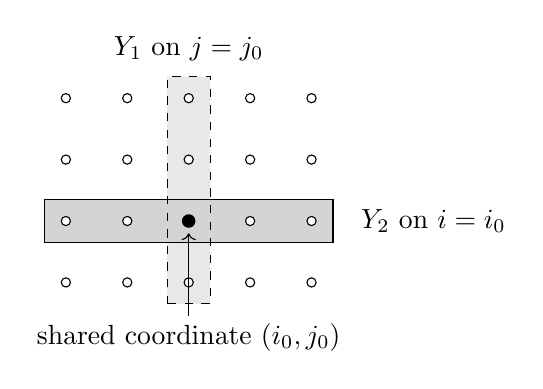
\begin{tikzpicture}[scale=.78]
 \fill[black!9] (2.65,.65) rectangle (3.35,4.35);
 \fill[black!17] (.65,1.65) rectangle (5.35,2.35);
 \draw[dashed] (2.65,.65) rectangle (3.35,4.35);
 \draw (.65,1.65) rectangle (5.35,2.35);
 \foreach \i in {1,...,4} {
   \foreach \j in {1,...,5} {
     \fill[white] (\j,\i) circle (.075);
     \draw (\j,\i) circle (.075);
   }
 }
 \fill (3,2) circle (.11);
 \node at (3,4.8) {$Y_1$ on $j=j_0$};
 \node[anchor=west] at (5.65,2) {$Y_2$ on $i=i_0$};
 \node at (3,.1) {shared coordinate $(i_0,j_0)$};
 \draw[->] (3,.45)--(3,1.8);
\end{tikzpicture}
\caption{The selected tensor fibers share exactly one coordinate.
Their two-call product fixes the $(a-1)(b-1)$ coordinates outside
the cross. Other calls of the tensor word occur before or after this
consecutive pair.}
\label{pivot:fig:tensor-grid}
\end{figure}

\begin{lemma}[Scalar pivot invariance]\label{lem:scalar-pivot}
Under the hypotheses of \cref{lem:pivot-bound}, if $r=1$, then
$p(\widetilde K)=p(K)$.
\end{lemma}

\begin{proof}
Write $D=d\ne0$. For each positive integer $\ell$, use $\ell$
copies of $K$, with fresh data groups $x_1,\ldots,x_\ell$ of width
$n$ and one shared state coordinate. In chronological order the
recurrences are
\begin{equation}\label{pivot:eq:chain-forward}
 y_j=Ax_j+Cw_{j-1},\qquad
 w_j=Bx_j+dw_{j-1},\qquad 1\le j\le\ell.
\end{equation}
Let $\mathcal C_\ell$ send
$(x_1,\ldots,x_\ell,w_0)$ to
$(y_1,\ldots,y_\ell,w_\ell)$. At every extension the previous
chain is regarded as a matrix only on its old data groups and its
one state coordinate. The next data group is outside this set, so
the intersection with the next call is exactly the one state
coordinate. Coordinates fixed by the old chain remain members of
its old set; no padding from the tensor-grid proof is added to it.
Induction using \cref{pivot:lem:one-port} gives
\begin{equation}\label{pivot:eq:forward-chain-price}
 p(\mathcal C_\ell)=\ell p(K).
\end{equation}

The full chain is invertible as a product of invertible calls. Its
state-to-state block is $d^\ell$, and its direct block on the data is
lower block triangular with diagonal blocks $A$. In fact its
$(j,i)$ block for $i<j$ is $Cd^{j-1-i}B$, and its blocks for $i>j$
vanish. Both blocks required by \cref{lem:pivot-bound} are therefore
invertible for every $\ell$.

Pivoting the boundary state means that $w_\ell$ is given and $w_0$
is requested. The exact backward recurrence is
\begin{equation}\label{pivot:eq:chain-backward}
 w_{j-1}=d^{-1}w_j-d^{-1}Bx_j,\qquad
 y_j=(A-Cd^{-1}B)x_j+Cd^{-1}w_j.
\end{equation}
Thus the pivoted chain $\widetilde{\mathcal C}_\ell$ consists of
copies of $\widetilde K$ in the order $j=\ell,\ldots,1$, again
with fresh data groups and one shared state. The same intersection
argument gives
\begin{equation}\label{pivot:eq:reverse-chain-price}
 p(\widetilde{\mathcal C}_\ell)=\ell p(\widetilde K).
\end{equation}
Put $S=A-Cd^{-1}B$. Since $\det K=d\det S$, the matrix $S$ is
invertible. The reverse chain has state block $d^{-\ell}$ and a
direct data block upper triangular in chronological order, with
diagonal blocks $S$; equivalently it is lower triangular in reverse
chronological order. Its full matrix is invertible too. Hence
\cref{lem:pivot-bound} applies both to the forward chain and to
the reverse chain. Pivoting the reverse chain returns the forward
chain, and therefore
\[
 \ell p(\widetilde K)\le\ell p(K)+4,
 \qquad
 \ell p(K)\le\ell p(\widetilde K)+4.
\]
Equivalently, $|p(\widetilde K)-p(K)|\le4/\ell$ for every $\ell$.
Letting $\ell$ tend to infinity proves equality. The earlier pivot
inequality is an exact statement for each finite matrix, so this
argument requires no estimate uniform in the increasing data width.
\end{proof}

\begin{corollary}[Exchange of two basis members]
\label{pivot:cor:basis-exchange}
Let $U=(u_1,\ldots,u_n,u_*)$ and
$V=(v_1,\ldots,v_n,v_*)$ be ordered bases of the same space of
linear forms, viewing each list as a column vector of its forms, and let
\[
 V=KU,\qquad K=\begin{pmatrix}A&C\\B&d\end{pmatrix}.
\]
The exchanged lists
\[
 U'=(u_1,\ldots,u_n,v_*),\qquad
 V'=(v_1,\ldots,v_n,u_*)
\]
are both bases if and only if $d\ne0$ and $\det A\ne0$.
Whenever this holds, the transitions $U\mapsto V$ and
$U'\mapsto V'$ have equal price. The statement applies to any
chosen member of each basis after reordering them to the last
positions.
\end{corollary}

\begin{proof}
Relative to $U$, the coefficient matrices of $U'$ and $V'$ are
\[
 \begin{pmatrix}\Id_n&0\\ B&d\end{pmatrix},\qquad
 \begin{pmatrix}A&C\\0&1\end{pmatrix},
\]
with determinants $d$ and $\det A$, respectively. These give the
asserted criterion exactly. When both are nonzero, the transition
between them is \cref{pivot:eq:pivot-matrix} with scalar pivot.
Apply \cref{lem:scalar-pivot}. Reorderings have zero price.
\end{proof}

\subsection{Four forms and the dense-pair bound}

\begin{lemma}[Price of a dense pair]\label{lem:pair-price}
Every invertible $2\times2$ matrix all of whose entries are nonzero
has price at most $3/2$. In particular,
\begin{equation}\label{pivot:eq:pair-bound}
 p\left(\begin{pmatrix}1&1\\1&u\end{pmatrix}\right)
 \le\frac32\qquad (u\in\C\setminus\{0,1\}).
\end{equation}
\end{lemma}

\begin{proof}
For a pair matrix $H$, the tensor law reads
$p(H\otimes H)=4p(H)$. We therefore seek a four-coordinate map
of price at most six that becomes a tensor square after monomial
changes. Two shears and the basis exchanges below put this map into
the form of a rank-one perturbation of the identity, making the
required monomial changes explicit.

Fix $\lambda\in\C\setminus\{0,1\}$ and four independent linear
forms $a,b,c,d$. We first bound the transition from
\[
 Y^{(0)}=(a,b,c,d)\quad\hbox{to}\quad
 X=(a+b,b+c,c+d,d+\lambda a).
\]
Its matrix is $\Id_4+J$, where
\[
 J=\begin{pmatrix}
 0&1&0&0\\0&0&1&0\\0&0&0&1\\\lambda&0&0&0
 \end{pmatrix},\qquad J^4=\lambda\Id_4.
\]
Here $J$ is monomial because $\lambda\ne0$, and
\[
 (\Id_4+J)(\Id_4-J+J^2-J^3)=(1-\lambda)\Id_4
\]
shows that $\Id_4+J$ is invertible. Apply
\cref{thm:feedback} at parameter one to
\[
 \mathcal L=\begin{pmatrix}\Id_4&J\\\Id_4&0\end{pmatrix}.
\]
This full cell is invertible, its direct block and feedback
denominator are identities, and its output is $\Id_4+J$.
To implement $\mathcal L$, send $(h,l)$ to $(h,Jl)$ by a monomial,
add $h_i$ into the second coordinate of each of the four pairs,
and swap the two blocks. Consequently
\begin{equation}\label{pivot:eq:four-start}
 p(\Id_4+J)\le p(\mathcal L)\le4.
\end{equation}

We change the first and third members on the $Y$ side using two
shears and legal exchanges. For clarity, all intermediate lists
are displayed below. Put
\[
 X_b=(a+b,b,c+d,d+\lambda a),\qquad
 X_d=(a+b,b+c,c+d,d).
\]
Every determinant in the last two columns is computed from the
coefficient rows in the original ordered basis $(a,b,c,d)$.
\begin{center}
\small
\begin{tabular}{@{}c l c c c@{}}
\toprule
Stage & $Y$ list & $X$ list & $\det Y$ & $\det X$\\
\midrule
0 & $(a,b,c,d)$ & $X$ & $1$ & $1-\lambda$\\
1 & $(a,b+c,c,d)$ & $X_b$ & $1$ & $1$\\
2 & $(a+b+c,b+c,c,d)$ & $X_b$ & $1$ & $1$\\
3 & $(a+b+c,b,c,d)$ & $X$ & $1$ & $1-\lambda$\\
4 & $(a+b+c,b,c,d+\lambda a)$ & $X_d$ & $1$ & $1$\\
5 & $(a+b+c,b,c+d+\lambda a,d+\lambda a)$
  & $X_d$ & $1$ & $1$\\
6 & $(a+b+c,b,c+d+\lambda a,d)$
  & $X$ & $1-\lambda$ & $1-\lambda$\\
\bottomrule
\end{tabular}
\end{center}
The steps $0\to1$ and $2\to3$ exchange the second members;
the steps $3\to4$ and $5\to6$ exchange the fourth members.
The step $1\to2$ adds the second member of $Y$ into its first,
and $4\to5$ adds its fourth member into its third. These are
the only two shears. The determinant table proves that every list
is a basis, including on both sides of every exchange; it follows
also by direct elementary row operations. Thus
\cref{pivot:cor:basis-exchange} applies at all four exchanges.
Changing the source basis from $Y$ to $EY$ by a shear replaces its
transition matrix $T$ by $TE^{-1}$, increasing price by at most one.
Together with \cref{pivot:eq:four-start}, this proves that the
transition from the last $Y$ list to $X$ has price at most six.

Reorder these final lists as
\[
 \overline Y=(a+b+c,b,d,c+d+\lambda a),\qquad
 \overline X=(b+c,b+a,d+\lambda a,c+d).
\]
Let
\[
 k=(1,-1,1,-1)^{\mathsf T},\qquad
 \Delta=(-1,1,\lambda,-\lambda)^{\mathsf T}.
\]
Then $k^{\mathsf T}\overline Y=(1-\lambda)a$ and
$\overline X-\overline Y=\Delta a$, so the transition matrix is
the explicit rank-one perturbation
\begin{equation}\label{pivot:eq:rank-one}
 T=\Id_4+\frac{\Delta k^{\mathsf T}}{1-\lambda},
 \qquad p(T)\le6.
\end{equation}

We now give the diagonal scalings. All their entries are nonzero
under the stated hypotheses on $\lambda$. Set $u=\lambda^{-1}$ and
\[
 L_1=\diag\left(\frac{1-\lambda}{\Delta_1},
 \frac{1-\lambda}{\Delta_2},
 \frac{1-\lambda}{\Delta_3},
 \frac{1-\lambda}{\Delta_4}\right),\qquad
 R_1=\diag(1,-1,1,-1).
\]
The rank-one summand of $L_1TR_1$ has every entry equal to one,
and a direct calculation gives
\[
 L_1TR_1=
 \begin{pmatrix}
 \lambda&1&1&1\\1&\lambda&1&1\\
 1&1&u&1\\1&1&1&u
 \end{pmatrix}.
\]
With the further scalings
\[
 L_2=\diag(u,u,u,1),\qquad R_2=\diag(1,1,1,\lambda),
\]
we obtain
\begin{equation}\label{pivot:eq:tensor-rescaling}
 L_2L_1TR_1R_2=
 \begin{pmatrix}
 1&u&u&1\\u&1&u&1\\u&u&u^2&1\\1&1&1&1
 \end{pmatrix}.
\end{equation}
Write $B(u)=\left(\begin{smallmatrix}1&1\\1&u\end{smallmatrix}\right)$.
The $(\alpha,\gamma)$ entry of $B(u)\otimes B(u)$, for bit pairs
$\alpha,\gamma\in\{0,1\}^2$, is
$u^{\alpha_1\gamma_1+\alpha_2\gamma_2}$.
Ordering its rows by $10,01,11,00$ and its columns by
$01,10,11,00$ gives exactly \cref{pivot:eq:tensor-rescaling}.
All the scalings and permutations preserve price. The tensor law
therefore yields
\[
 4p(B(u))=p(B(u)\otimes B(u))=p(T)\le6.
\]
Every $u\ne0,1$ arises from the permitted choice $\lambda=1/u$,
proving \cref{pivot:eq:pair-bound}.

Finally, if $H=\left(\begin{smallmatrix}a&b\\c&d\end{smallmatrix}\right)$
is dense and invertible, then
\[
 \diag(a^{-1},c^{-1})\,H\,\diag(1,a/b)
 =B\left(\frac{ad}{bc}\right).
\]
Density makes $ad/(bc)\ne0$, and invertibility makes it different
from one. Monomial invariance completes the proof.
\end{proof}

\section{Signed matrices and the reflection contradiction}
\label{reflect:section}

We continue under the assumption that there is no finite win.  Thus the
price function of \cref{thm:prices}, the feedback and specialization laws,
and the pivot laws all apply.  We construct a real involution with a large
price and then use the orthogonal reflection in its positive eigenspace
to obtain incompatible price bounds.  All dimensions in the two
specializations below are fixed before either specialization is made.

\subsection{Signed bit operators with an exact price}

On one bit, set
\[
 C=\begin{pmatrix}0&0\\1&0\end{pmatrix},\qquad
 Z=\begin{pmatrix}1&0\\0&-1\end{pmatrix},\qquad
 X=\begin{pmatrix}0&1\\1&0\end{pmatrix}.
\]
For $m\geq 1$, define matrices on $m$ bits by
\begin{equation}
 D_1=C,\qquad
 D_{m+1}=C\otimes I_{2^m}+Z\otimes D_m
       =\begin{pmatrix}D_m&0\\ I_{2^m}&-D_m\end{pmatrix},
 \qquad T_m=I_{2^m}+D_m.
 \label{reflect:signed-recursion}
\end{equation}
The matrices $D_m$ are strictly lower triangular in lexicographic bit
order.  Squaring the displayed block matrix shows inductively that
$D_m^2=0$.  In particular, $T_m$ is invertible and
$T_m^{-1}=I_{2^m}-D_m$.

The signed tensor summands in this recursion have the standard
Jordan--Wigner creation-operator form, with tensor factors in the reverse
order of the convention in
\citet[Section~II.B, Equations~(10)--(11)]{seeleyRichardLove2012}.
Here the bits label ordinary matrix coordinates. The recursion above
and the price arguments below provide all identities needed for the
proof.

\begin{lemma}
\label{reflect:triangular-price}
For every integer $m\geq1$,
\[
 p(T_m)=m2^{m-1}.
\]
\end{lemma}

\begin{proof}
We have $T_1=U$, so $p(T_1)=1$.  Put $n=2^m$ and consider the transition
from input forms $x=(x_1,\ldots,x_{2n})$ to output forms $y=K_0x$, where
\[
 K_0=U\otimes T_m
     =\begin{pmatrix}T_m&0\\ T_m&T_m\end{pmatrix}.
\]
We shall exchange each bottom input form with the corresponding bottom
output form, using only the exact \emph{scalar} pivot law of
\cref{lem:scalar-pivot}.  Here is a determinant check for every
intermediate exchange.

For any subset $H\subseteq\{n+1,\ldots,2n\}$ of already exchanged
positions, keep the forms in their original index positions and set
\[
 u_i=\begin{cases}y_i&i\in H,\\x_i&i\notin H,\end{cases}
 \qquad
 v_i=\begin{cases}x_i&i\in H,\\y_i&i\notin H.\end{cases}
\]
Let $U_H,V_H$ be their coefficient matrices relative to $x$.
Simultaneously permuting rows and columns to put $H$ first gives
\[
 U_H\sim
 \begin{pmatrix}K_0[H,H]&K_0[H,H^c]\\0&I\end{pmatrix},\qquad
 V_H\sim
 \begin{pmatrix}I&0\\K_0[H^c,H]&K_0[H^c,H^c]\end{pmatrix}.
\]
The row and column permutation signs cancel.  Every principal submatrix
of the unit lower triangular matrix $K_0$ is unit lower triangular, so
\begin{equation}
 \det U_H=\det K_0[H,H]=1,
 \qquad
 \det V_H=\det K_0[H^c,H^c]=1.
 \label{reflect:mixed-minors}
\end{equation}
The empty principal minor, when it occurs, has determinant one.
Thus both lists are bases and their current transition
$Q_H=V_HU_H^{-1}$ has determinant one.

For the next index $j\notin H$ in the bottom half, replacing $u_j$ by
$v_j$ changes the input determinant by the factor $(Q_H)_{jj}$.
Replacing $v_j$ by $u_j$ changes the output determinant by
$(Q_H^{-1})_{jj}$.  Applying \eqref{reflect:mixed-minors} to $H$ and
$H\cup\{j\}$ therefore gives
\[
 (Q_H)_{jj}=\frac{\det U_{H\cup\{j\}}}{\det U_H}=1,
 \qquad
 (Q_H^{-1})_{jj}=\frac{\det V_{H\cup\{j\}}}{\det V_H}=1.
\]
Move position $j$ to the last port in both bases.  The scalar diagonal
block required for the pivot is consequently one; the determinant of
its complementary principal block is, by the cofactor identity,
\[
 \det Q_H\,(Q_H^{-1})_{jj}=1.
\]
Both hypotheses of \cref{lem:scalar-pivot} hold at every step, and each
exchange preserves the price exactly.

After all bottom positions have been exchanged, write the original
inputs as $(a,b)$ and the bottom output as $z=T_ma+T_mb$.
Solving gives $b=T_m^{-1}z-a$.  Thus the final transition, from $(a,z)$
to $(T_ma,b)$, is
\[
 \begin{pmatrix}T_m&0\\-I&T_m^{-1}\end{pmatrix}.
\]
Conjugating by $\diag(I,-I)$ changes the lower left block to $I$;
the result is $T_{m+1}$ by \eqref{reflect:signed-recursion}.
Monomial invariance and the tensor law now give
\[
 p(T_{m+1})=p(U\otimes T_m)=2^m+2p(T_m),
\]
which proves the formula by induction.
\end{proof}

Fix an integer $d\geq1$.  On $d+1$ bits, of width $N=2^{d+1}$, put
\begin{equation}
 \Gamma=X\otimes I_{2^d}+Z\otimes D_d
       =\begin{pmatrix}D_d&I\\I&-D_d\end{pmatrix}.
 \label{reflect:gamma}
\end{equation}
Since $D_d^2=0$, this is a real involution.  Its price is also exact:
\begin{equation}
 p(\Gamma)=\frac{dN}{2}.
 \label{reflect:gamma-price}
\end{equation}
To verify this, multiplication on the left by the monomial
$X\otimes I$ gives $I+(XZ)\otimes D_d$.
The recursion expands as
\[
 D_d=\sum_{i=1}^d
       Z^{\otimes(i-1)}\otimes C\otimes I_{2^{d-i}}.
\]
Each nonzero entry therefore changes exactly one bit from zero to one,
increasing Hamming weight by one.  Define the signed monomial $P$ to
act on the first bit by $(XZ)^{-|b|}$ when the last $d$ bits have value
$b$ and Hamming weight $|b|$.  On a transition of these last bits from
weight $j$ to weight $j+1$, conjugation by $P$ changes the first-bit
factor to
\[
 (XZ)^{-(j+1)}(XZ)(XZ)^j=I_2.
\]
It leaves the identity term unchanged.  Hence
\[
 P\bigl(I+(XZ)\otimes D_d\bigr)P^{-1}=I_2\otimes T_d,
\]
and \eqref{reflect:gamma-price} follows from
\cref{reflect:triangular-price} and the tensor law.

We next record a transpose symmetry.  Define the signed orthogonal
monomial
\begin{equation}
 J=\bigotimes_{i=1}^{d+1}(Z^{i-1}X).
 \label{reflect:j-definition}
\end{equation}
For its $i$th factor $H_i=Z^{i-1}X$, direct multiplication gives
\[
 H_i^{\mathsf T}=(-1)^{i-1}H_i,\qquad
 H_iZH_i^{-1}=-Z,\qquad
 H_iCH_i^{-1}=(-1)^{i-1}C^{\mathsf T}.
\]
The first-bit term of $\Gamma$ is $X\otimes I$ and is fixed by this
conjugation.  Every other term has the form
\[
 Z^{\otimes(i-1)}\otimes C\otimes I_{2^{d+1-i}},
 \qquad 2\leq i\leq d+1.
\]
The $i-1$ prefix signs and the sign from the $C$ factor cancel.  It
follows that
\begin{equation}
 J\Gamma J^{-1}=\Gamma^{\mathsf T},\qquad
 J^{\mathsf T}=(-1)^{d(d+1)/2}J.
 \label{reflect:transpose-symmetry}
\end{equation}

On width $w=N^2$, set
\begin{equation}
 M=\Gamma\otimes\Gamma,\qquad
 L=\Gamma\otimes I_N-I_N\otimes\Gamma,\qquad
 S=J\otimes J,\qquad A=SL.
 \label{reflect:large-operators}
\end{equation}
The matrix $S$ is a symmetric orthogonal monomial, so $S^{-1}=S$.
Equation~\eqref{reflect:transpose-symmetry} gives
$SLS^{-1}=L^{\mathsf T}$, and consequently
\[
 A^{\mathsf T}=L^{\mathsf T}S^{\mathsf T}=SL=A.
\]
In particular, $A$ is real symmetric.  Moreover,
\begin{equation}
 (\Gamma\otimes I_N)L=I_w-M,
 \qquad
 E:=\ker A=\ker L=\ker(I_w-M).
 \label{reflect:kernel}
\end{equation}
Thus $E$ is the positive eigenspace of the involution $M$.

We shall need a count of the supported unordered off-diagonal pairs
of $A$.  The first-bit flip in $\Gamma$ has $N$ nonzero entries, and
each of its other $d$ bit terms has $N/2$ nonzero entries.  Their
supports are disjoint, since they change different bits.  Thus
$\nnz(\Gamma)=(1+d/2)N$.
The supports of $\Gamma\otimes I_N$ and $I_N\otimes\Gamma$ are
also disjoint: they change a bit in different tensor factors.
Therefore
\[
 \nnz(L)=(d+2)w,\qquad \nnz(A)=(d+2)w.
\]
Symmetry makes every supported off-diagonal pair account for two
entries.  If $h$ is the number of such pairs, we have
\begin{equation}
 h\leq (d/2+1)w.
 \label{reflect:pair-count}
\end{equation}

Let $R$ be the orthogonal reflection in $E$. The rest of the argument
will establish the bounds
\[
 (d-4)w\leq p(R)\leq
 \left(\frac{3d}{4}+\frac72\right)w.
\]
They are incompatible when $d>30$.
The upper bound uses the description $E=\ker A$: a polynomial
perturbation has one dense pair factor of price at most $3/2$ for
each supported pair of $A$, at generic parameter values. Two algebraic
specializations turn this bound into a price for the reflection.
The lower bound uses $E$ as the positive eigenspace of $M$, whose
tensor price is $dw$.
Its graph description will recover the full price of $M$ from $R$, at
a cost of at most $4w$. Thus the contradiction comes from the different
coefficients of $d$, while the changes of boundary coordinates cost
only a fixed multiple of the width.

\subsection{Pricing a reflection by two algebraic specializations}

The following statement isolates the use of sparsity.  Orthogonality
refers to the usual real inner product; all real maps and subspaces
are then complexified when their prices are taken.

\begin{lemma}
\label{reflect:sparse-reflection}
Let $A$ be a real symmetric $w\times w$ matrix with $h$ supported
unordered off-diagonal pairs.  Let $R$ act as $+I$ on $\ker A$ and
as $-I$ on $(\ker A)^\perp$.  Then
\[
 p(R)\leq \frac32h+2w.
\]
\end{lemma}

\begin{proof}
Write $e_{ij}$ for matrix units, and fix any order of the supported
pairs.  Form the polynomial matrix
\begin{equation}
 K(\eps)=\left(I+\eps\diag(A_{11},\ldots,A_{ww})\right)
       \prod_{\substack{i<j\\A_{ij}\ne0}}
       \left(I+\eps A_{ij}(e_{ij}+e_{ji})\right).
 \label{reflect:polynomial-product}
\end{equation}
Then $K(0)=I$ and $K'(0)=A$.  Outside a finite set $E_0$,
the diagonal factor is an invertible monomial and every other factor
acts on its two coordinates as the dense invertible matrix
\[
 \begin{pmatrix}1&\eps A_{ij}\\\eps A_{ij}&1\end{pmatrix}.
\]
For example, $E_0$ may contain zero, the roots of the diagonal-factor
determinant, and all roots of $1-\eps^2A_{ij}^2$ for the supported
pairs.  These are finitely many roots of nonzero polynomials.
By \cref{lem:pair-price}, direct sums, and product subadditivity,
\begin{equation}
 p(K(\eps))\leq \frac32h\qquad(\eps\notin E_0).
 \label{reflect:product-price}
\end{equation}

Put $Q(\eps)=(K(\eps)-I)/\eps$, with its polynomial extension
$Q(0)=A$.  First fix a parameter $t$ outside the single finite set
\begin{equation}
 \mathcal E=\{0\}\cup
 \{\lambda^{-1},-\lambda^{-1}:
                    \lambda\in\operatorname{spec}(A),\ \lambda\ne0\}.
 \label{reflect:outer-exceptions}
\end{equation}
The polynomial matrices
\[
 C_+(\eps)=I+tQ(\eps),\qquad C_-(\eps)=I-tQ(\eps)
\]
have nonzero determinants at zero, since $I\pm tA$ are invertible.
Consequently the rational output
\[
 H_t(\eps)=C_+(\eps)C_-(\eps)^{-1}
\]
is regular and invertible at zero.

For this fixed $t$, exclude also $\eps=0,t,-t$ and the roots of
$\det C_+(\eps)\det C_-(\eps)$, in addition to $E_0$.
This defines a finite set $E_t$, which may depend on $t$.
For $\eps\notin E_t$ define
\[
 m=\frac{\eps-t}{\eps+t},\qquad
 s=\frac{t}{\eps+t},\qquad
 v=\frac{2\eps t}{(\eps+t)^2},
\]
and consider the data--state cell
\begin{equation}
 F_{t,\eps}=
 \begin{pmatrix}mI_w&K(\eps)\\vI_w&sK(\eps)\end{pmatrix}
 =\begin{pmatrix}mI_w&I_w\\vI_w&sI_w\end{pmatrix}
   \diag(I_w,K(\eps)).
 \label{reflect:feedback-cell}
\end{equation}
The first factor is a direct sum, after reordering, of $w$ scalar
pair matrices.  Their determinants are
\[
 ms-v=-\frac{t}{\eps+t}\ne0.
\]
Hence the cell is invertible.  Its direct block $mI_w$ is invertible,
and its feedback denominator at feedback parameter one satisfies
\begin{equation}
 I_w-sK(\eps)=\frac{\eps}{\eps+t}C_-(\eps),
 \label{reflect:feedback-denominator}
\end{equation}
so that denominator is invertible too.  Its feedback output is exactly
\begin{align*}
 mI_w+K(\eps)(I_w-sK(\eps))^{-1}v
 &=\bigl(mI_w+(v-ms)K(\eps)\bigr)
                         (I_w-sK(\eps))^{-1}\\
 &=C_+(\eps)C_-(\eps)^{-1}=H_t(\eps).
\end{align*}
The last equality follows from
$mI_w+(v-ms)K(\eps)=\eps C_+(\eps)/(\eps+t)$.
The output is invertible by the choice of $E_t$, so every hypothesis
of \cref{thm:feedback} is satisfied.

An invertible scalar pair has price at most two.  The factorization
\eqref{reflect:feedback-cell} and \eqref{reflect:product-price}
therefore imply
\[
 p(H_t(\eps))\leq p(F_{t,\eps})
              \leq p(K(\eps))+2w
              \leq \frac32h+2w
              \qquad(\eps\notin E_t).
\]
Apply \cref{thm:specialization} to the rational matrix $H_t$ at
$\eps=0$.  This proves
\begin{equation}
 p\bigl((I+tA)(I-tA)^{-1}\bigr)\leq C_A,
 \qquad C_A=\frac32h+2w,
 \qquad t\notin\mathcal E.
 \label{reflect:first-specialization}
\end{equation}
The quantifiers here are useful: $A,w,h$ and $C_A$ were fixed first;
for \emph{each} $t\notin\mathcal E$ there is a finite $E_t$ giving
the same bound, and specialization is applied separately for that
$t$.  Thus \eqref{reflect:first-specialization} holds for every
$t$ outside one finite set, with one price bound.
Only the rational output is specialized.  At $\eps=0$ the cell
itself would have $m=-1$, $s=1$, $v=0$, and $K=I$, making its
feedback denominator zero; no feedback law is applied to that cell.

For the second specialization use $z=1/t$ and the rational matrix
\[
 Y(z)=(zI_w+A)(zI_w-A)^{-1}.
\]
By the Real Spectral Theorem, $A=O\diag(\lambda_1,\ldots,\lambda_w)
O^{\mathsf T}$ for a real orthogonal $O$ and real eigenvalues
$\lambda_i$.  In this basis, the corresponding rational functions
are $(z+\lambda_i)/(z-\lambda_i)$.
If $\lambda_i=0$, this function is identically one after cancellation;
if $\lambda_i\ne0$, it is regular at zero with value minus one.
It follows that $Y$ is regular at zero and $Y(0)=R$, an invertible
matrix.  In particular, the zero eigenspace is semisimple; real
symmetry supplies exactly the diagonalizability needed for this
removable-singularity assertion.

For all $z$ outside
$\{0\}\cup\{\lambda,-\lambda:\lambda\in\operatorname{spec}(A),
\lambda\ne0\}$, we may take $t=1/z$ in
\eqref{reflect:first-specialization}.  Hence $p(Y(z))\leq C_A$
outside a finite set.  A second application of
\cref{thm:specialization} yields $p(R)\leq C_A$.
The orthogonal diagonalization was used to identify a rational
matrix and its value; it was not used as a priced implementation.
Neither specialization assumes continuity of $p$.
\end{proof}

Apply \cref{reflect:sparse-reflection} to $A=SL$ from
\eqref{reflect:large-operators}.  With $R$ the orthogonal reflection
in $E$ from \eqref{reflect:kernel}, \eqref{reflect:pair-count} gives
\begin{equation}
 p(R)\leq \frac32(d/2+1)w+2w
        =\left(\frac{3d}{4}+\frac72\right)w.
 \label{reflect:upper-bound}
\end{equation}

\subsection{The graph of the positive eigenspace}

Every nonzero term of $\Gamma$ changes exactly one bit, so $\Gamma$
anticommutes with the parity sign $\Pi=Z^{\otimes(d+1)}$.
Consequently $M$ anticommutes with $\Pi\otimes I_N$.
Order the coordinates according to this first-factor parity.
The two parts have equal width $r=w/2$, and in this order
\begin{equation}
 M=\begin{pmatrix}0&B\\B^{-1}&0\end{pmatrix}
 \quad\hbox{for some }B\in\GL_r(\R).
 \label{reflect:graph-involution}
\end{equation}
Indeed anticommutation forces the diagonal blocks to vanish, and
$M^2=I$ forces the two off-diagonal blocks to be mutual inverses.
The tensor law and \eqref{reflect:gamma-price} give
\begin{equation}
 p(M)=2N p(\Gamma)=dw=2p(B),
 \label{reflect:m-price}
\end{equation}
where the last equality follows by multiplying
\eqref{reflect:graph-involution} by a block-swap permutation and
then using direct sums and inverse symmetry.

Equation~\eqref{reflect:graph-involution} identifies
\[
 E=\{(Bv,v):v\in\R^r\},\qquad
 E^\perp=\{(u,v):B^{\mathsf T}u+v=0\}.
\]
Let $Q=I_r+B^{\mathsf T}B$.  For every nonzero real vector $v$,
$v^{\mathsf T}Qv=\|v\|^2+\|Bv\|^2>0$; hence $Q$ is invertible.
The columns of $\binom{B}{I_r}$ form a basis of $E$, so its
orthogonal projection is
\[
 P_E=\begin{pmatrix}B\\I_r\end{pmatrix}
       Q^{-1}\begin{pmatrix}B^{\mathsf T}&I_r\end{pmatrix}.
\]
As $R=2P_E-I_w$, its off-diagonal blocks in the parity order are
\begin{equation}
 R_{+,-}=2BQ^{-1},\qquad
 R_{-,+}=2Q^{-1}B^{\mathsf T}=R_{+,-}^{\mathsf T}.
 \label{reflect:invertible-offdiagonals}
\end{equation}
Both are invertible.  This use of positive definiteness is over
$\R$; all these invertible real matrices also define invertible
complex linear maps.

For $y=Rx$, order the input as $(x_-,x_+)$ and the output as
$(y_+,y_-)$.  The resulting transition is
\[
 K_R=\begin{pmatrix}R_{+,-}&R_{+,+}\\
                    R_{-,-}&R_{-,+}\end{pmatrix}.
\]
The two diagonal blocks required by \cref{lem:pivot-bound} are now
precisely the invertible blocks in
\eqref{reflect:invertible-offdiagonals}.
Pivot the second group of $r$ ports and then swap the two output
groups.  The resulting map
\[
 V:(x_-,y_-)\longmapsto(x_+,y_+)
\]
therefore satisfies
\begin{equation}
 p(V)\leq p(R)+4r.
 \label{reflect:graph-pivot-price}
\end{equation}

Since $R$ is the reflection in $E$, the vectors $x+y$ and $x-y$
belong to $E$ and $E^\perp$, respectively.  Their graph equations are
\[
 x_++y_+=B(x_-+y_-),\qquad
 x_+-y_+=-B^{-\mathsf T}(x_--y_-).
\]
For the invertible sum-and-difference map
\[
 F=\begin{pmatrix}I_r&I_r\\I_r&-I_r\end{pmatrix},
 \qquad F^{-1}=\tfrac12F,
\]
these equations state the exact identity
\begin{equation}
 FVF^{-1}=\diag(B,-B^{-\mathsf T}).
 \label{reflect:graph-diagonalization}
\end{equation}
The relation between the coordinates is displayed in
\cref{reflect:graph-figure}.

\begin{figure}[ht]
\centering
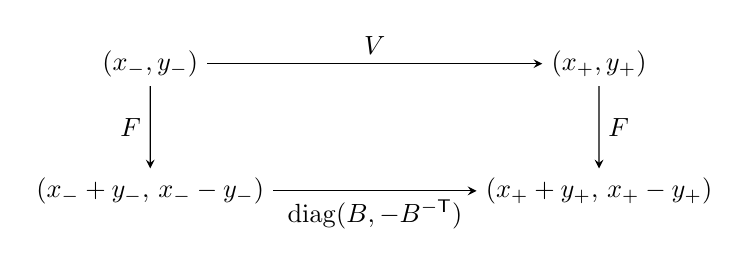
\begin{tikzpicture}[>=stealth, every node/.style={align=center},
                    scale=0.95, transform shape]
 \node (a) at (0,1.5) {$ (x_-,y_-) $};
 \node (b) at (6,1.5) {$ (x_+,y_+) $};
 \node (c) at (0,-0.2) {$ (x_-+y_-,\,x_--y_-) $};
 \node (e) at (6,-0.2) {$ (x_++y_+,\,x_+-y_+) $};
 \draw[->] (a) -- node[above] {$V$} (b);
 \draw[->] (a) -- node[left] {$F$} (c);
 \draw[->] (b) -- node[right] {$F$} (e);
 \draw[->] (c) -- node[below] {$\diag(B,-B^{-\mathsf T})$} (e);
\end{tikzpicture}
\caption{Pivoting the reflection exposes its two graph equations.
The sums are the parity components of $x+y\in E$; the differences
are the parity components of $x-y\in E^\perp$.
All four maps are exact invertible linear maps.}
\label{reflect:graph-figure}
\end{figure}

After interleaving coordinates, $F$ is a direct sum of $r$ invertible
scalar pair maps.  Thus $p(F)=p(F^{-1})\leq2r$.
Combining \eqref{reflect:m-price},
\eqref{reflect:graph-pivot-price}, and
\eqref{reflect:graph-diagonalization}, and using transpose and
inverse symmetry, yields
\begin{equation}
 dw=2p(B)
    =p\bigl(\diag(B,-B^{-\mathsf T})\bigr)
    \leq p(V)+4r
    \leq p(R)+8r
    =p(R)+4w.
 \label{reflect:lower-bound}
\end{equation}

\begin{theorem}[Existence of a finite win]
\label{thm:finite-win}
There exist an invertible nonmonomial matrix $A$ of a finite width
$q$, an integer $b\geq2$, and a word on exactly $q^b$ coordinates
implementing $A^{\otimes b}$ with monomials and fewer than
$bq^{b-1}$ calls to $A$.
\end{theorem}

\begin{proof}
If there were no finite win, the preceding construction and all its
price bounds would apply for every fixed integer $d\geq1$.
Equations~\eqref{reflect:upper-bound} and
\eqref{reflect:lower-bound} would imply
\[
 dw\leq\left(\frac{3d}{4}+\frac{15}{2}\right)w.
\]
Since $w>0$, this says $d\leq30$, contrary to choosing any fixed
integer $d>30$.  This contradiction proves the theorem.
\end{proof}

By \cref{prop:win-to-fourier}, the finite win of
\cref{thm:finite-win} supplies lengths $n_j\to\infty$ and exact
circuits in the stated scalar-gate model whose sizes $s_j$ satisfy
\[
 \frac{s_j}{n_j\log_2 n_j}\longrightarrow0.
\]
For every $c>0$ and every integer cutoff $n_0\geq2$, some $j$
therefore has $n_j\geq n_0$ and $s_j<c n_j\log_2 n_j$.
This proves the precise negative alternative in \cref{thm:main}.
The conclusion is nonuniform existence along an unbounded sequence;
the auxiliary price zero of monomials and the two specializations do
not alter the scalar gate costs or the exactness of those circuits.

\bibliographystyle{plainnat}
\bibliography{references}
\end{document}
